\section{Growth of non-axisymmetric modes without the influence of the
  planet}\label{linear1} 
In this section, the planet is introduced at $t=20P_0$ and 
its potential is switched on over $10P_0$. At $t=30P_0$ we switch off the
planet potential and azimuthally average the surface density, energy
and velocity fields. (At this point the planet has carved a partial
gap and the RWI has not yet occurred.) Effectively, we initialise the
disc with a gap profile. 
We then perturb the surface density in the outer disc ($r>r_p$) and continue to 
evolve the disc. We impose  sinusoidal perturbations with 
azimuthal wavenumbers $m\in[1,10]$ and random amplitudes within $\pm 0.01$
times the local surface density. 
This procedure allows us to analyse the growth of 
non-axisymmetric modes associated with the gap, but without
complications from non-axisymmetry arising directly from disc-planet
interaction (i.e. planet-induced wakes). 

Note that these `planet-off' simulations are not linear stability
calculations because the cooling term in our energy equation
restores the initial temperature profile corresponding to constant
$H/r=0.05$, rather than the heated gap edge. However, we will 
examine a nearly adiabatic simulation in \S\ref{adiabatic_section},
which is closer to a proper linear problem. 

Simulations here employ a resolution of $(N_r,N_{\phi})=(1024,2048)$
with open boundaries at $r=r_\mathrm{in}$ and
$r_\mathrm{out}=25r_\mathrm{in}$. We compare cases with
$\tilde{\beta}=0.1,1,10$ corresponding to fast, moderately, 
and slowly cooled discs. 

\subsection{Gap structure}
We first compare the gap structures formed by planet-disc
interaction as a function of the cooling time. The azimuthally-averaged 
gap profiles are shown in Fig. \ref{intial1D} for different values of 
$\tilde\beta$. Gaps formed with lower $\tilde\beta$ (faster cooling) 
are deeper with steeper gradients at the gap edges. Faster cooling rates also 
increase (decrease) the surface density maxima (minima). However, a
clean gap does not form in this short time period.%
%\footnote{We find the
% RWI begins to develop if the disc is evolved beyond $t\sim30P_0$}.

Increasing $\tilde\beta$ leads to higher disc aspect ratios $h=H/r$,
i.e. higher temperatures. Heating mostly occurs at the gap edges
due to planet-induced spiral shocks. Increasing the cooling timescale 
implies that this heat is retained in the disc. In the inviscid limit the gap
opening condition is $r_h\gtrsim H$ or $q\gtrsim 3h^3$
\citep{crida06}, which indicates that for hotter discs (higher
$h$), it becomes more difficult for a planet of fixed $q$ to open a
gap. This explains the shallower gaps in surface density when
$\tilde{\beta}$ is increased. 

%However, notice the gap structure
%changes most significantly for $\beta =0.1 \to 1.0$. For $\beta \geq
%1$  

The important consequence of a heated gap edge is that the
generalised vortensity profiles, $\tilde{\eta}$, becomes smoother with increasing
cooling times, with the extrema becoming less pronounced. Previous locally
isothermal disc-planet simulations show the RWI associated with PV
minima \citep{li05,lin10}. We can therefore expect the RWI to be associated with
minima in the generalised vortensity (corresponding to local surface
density maxima) in the non-isothermal case. Because the extrema are
less sharp, the RWI is expected to be weaker and the gap to be more
stable with longer cooling times.  


However, we remark that the change in the gap structure becomes less 
significant at long cooling times, as Fig. \ref{intial1D} shows that
the profiles with $\tilde{\beta}=1$ and $\tilde{\beta}=10$ are 
similar. This implies that the effect of cooling timescale on the
RWI through the set up of the gap profile, becomes less important for
large $\tilde{\beta}$. 
% or 'suggets that .... becomes unimportant for sufficiently large...' 

\begin{figure}
  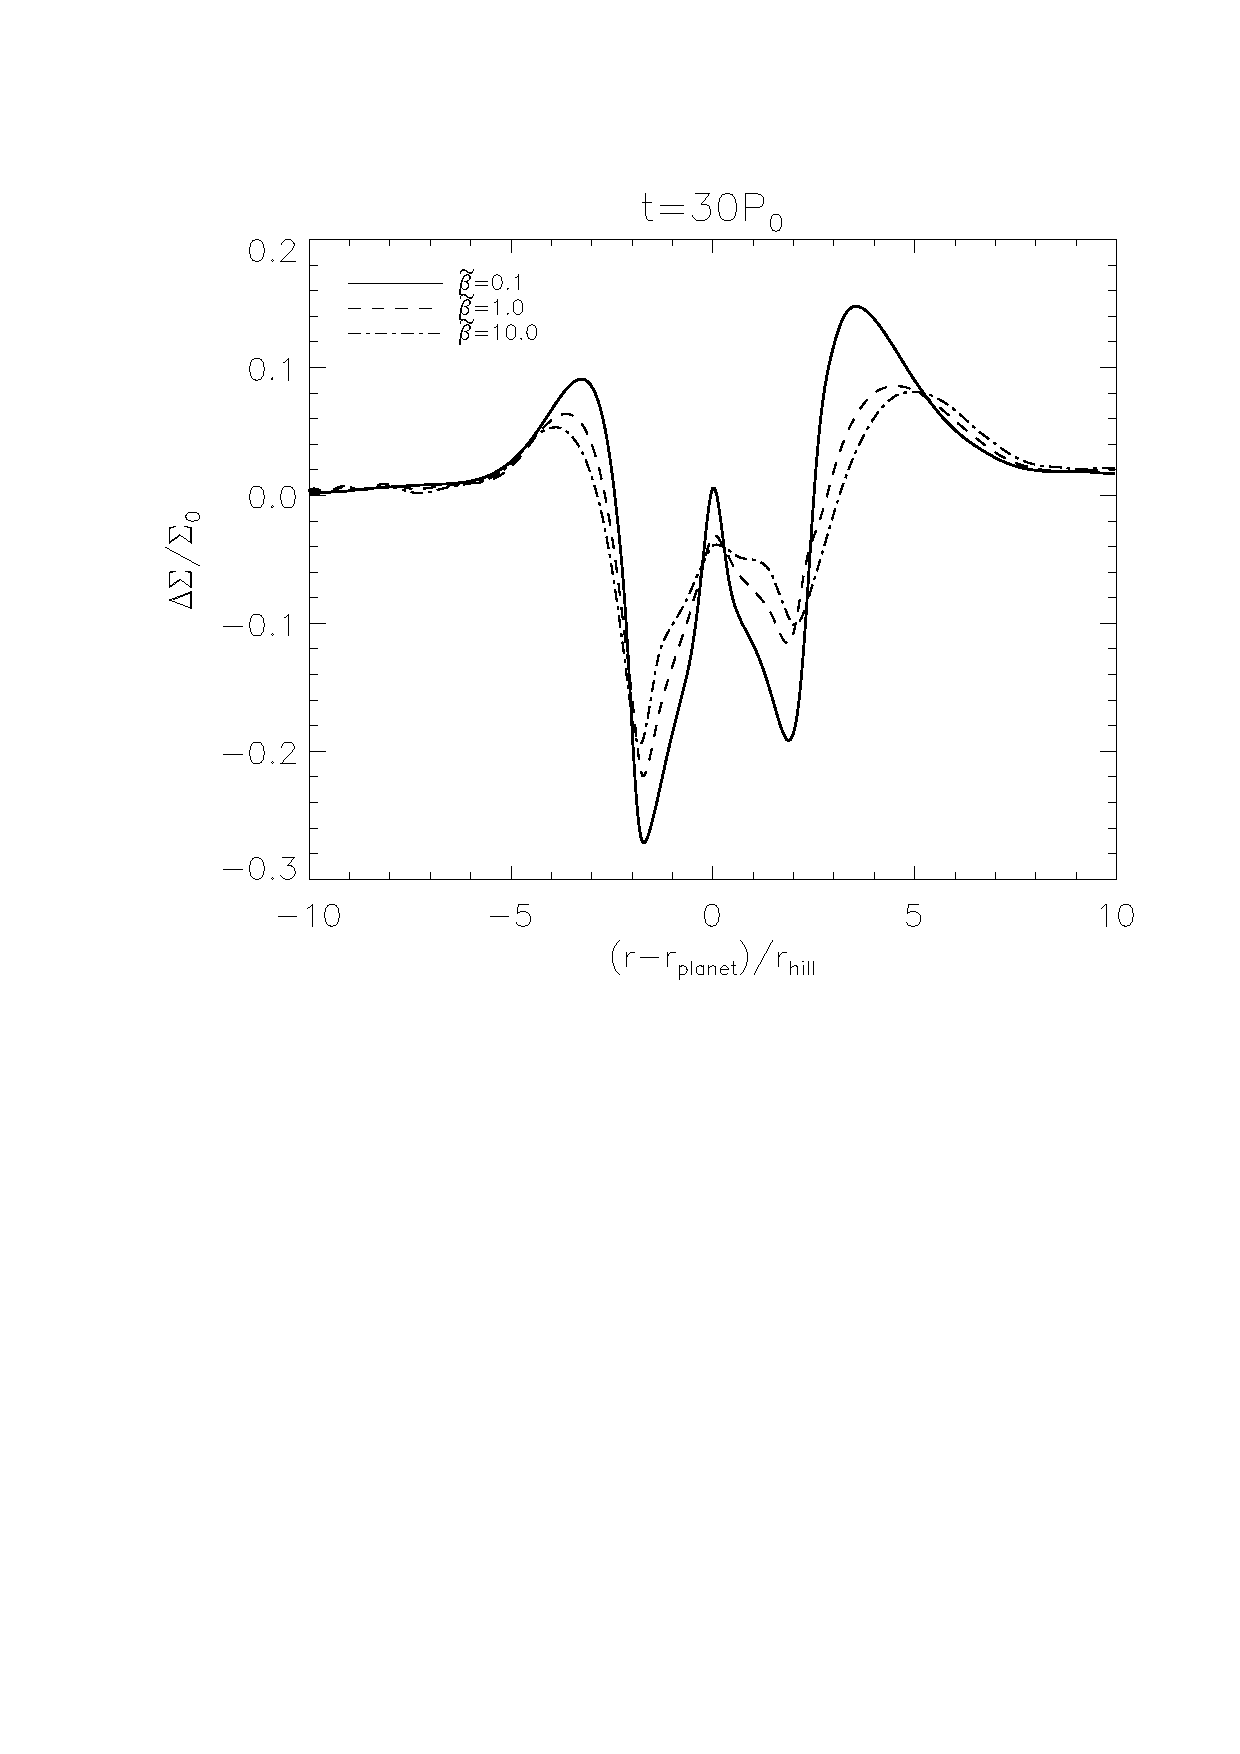
\includegraphics[width=\linewidth,clip=true,trim=0.5cm
    2cm 0cm 0cm]{figures/compare_sigma}
  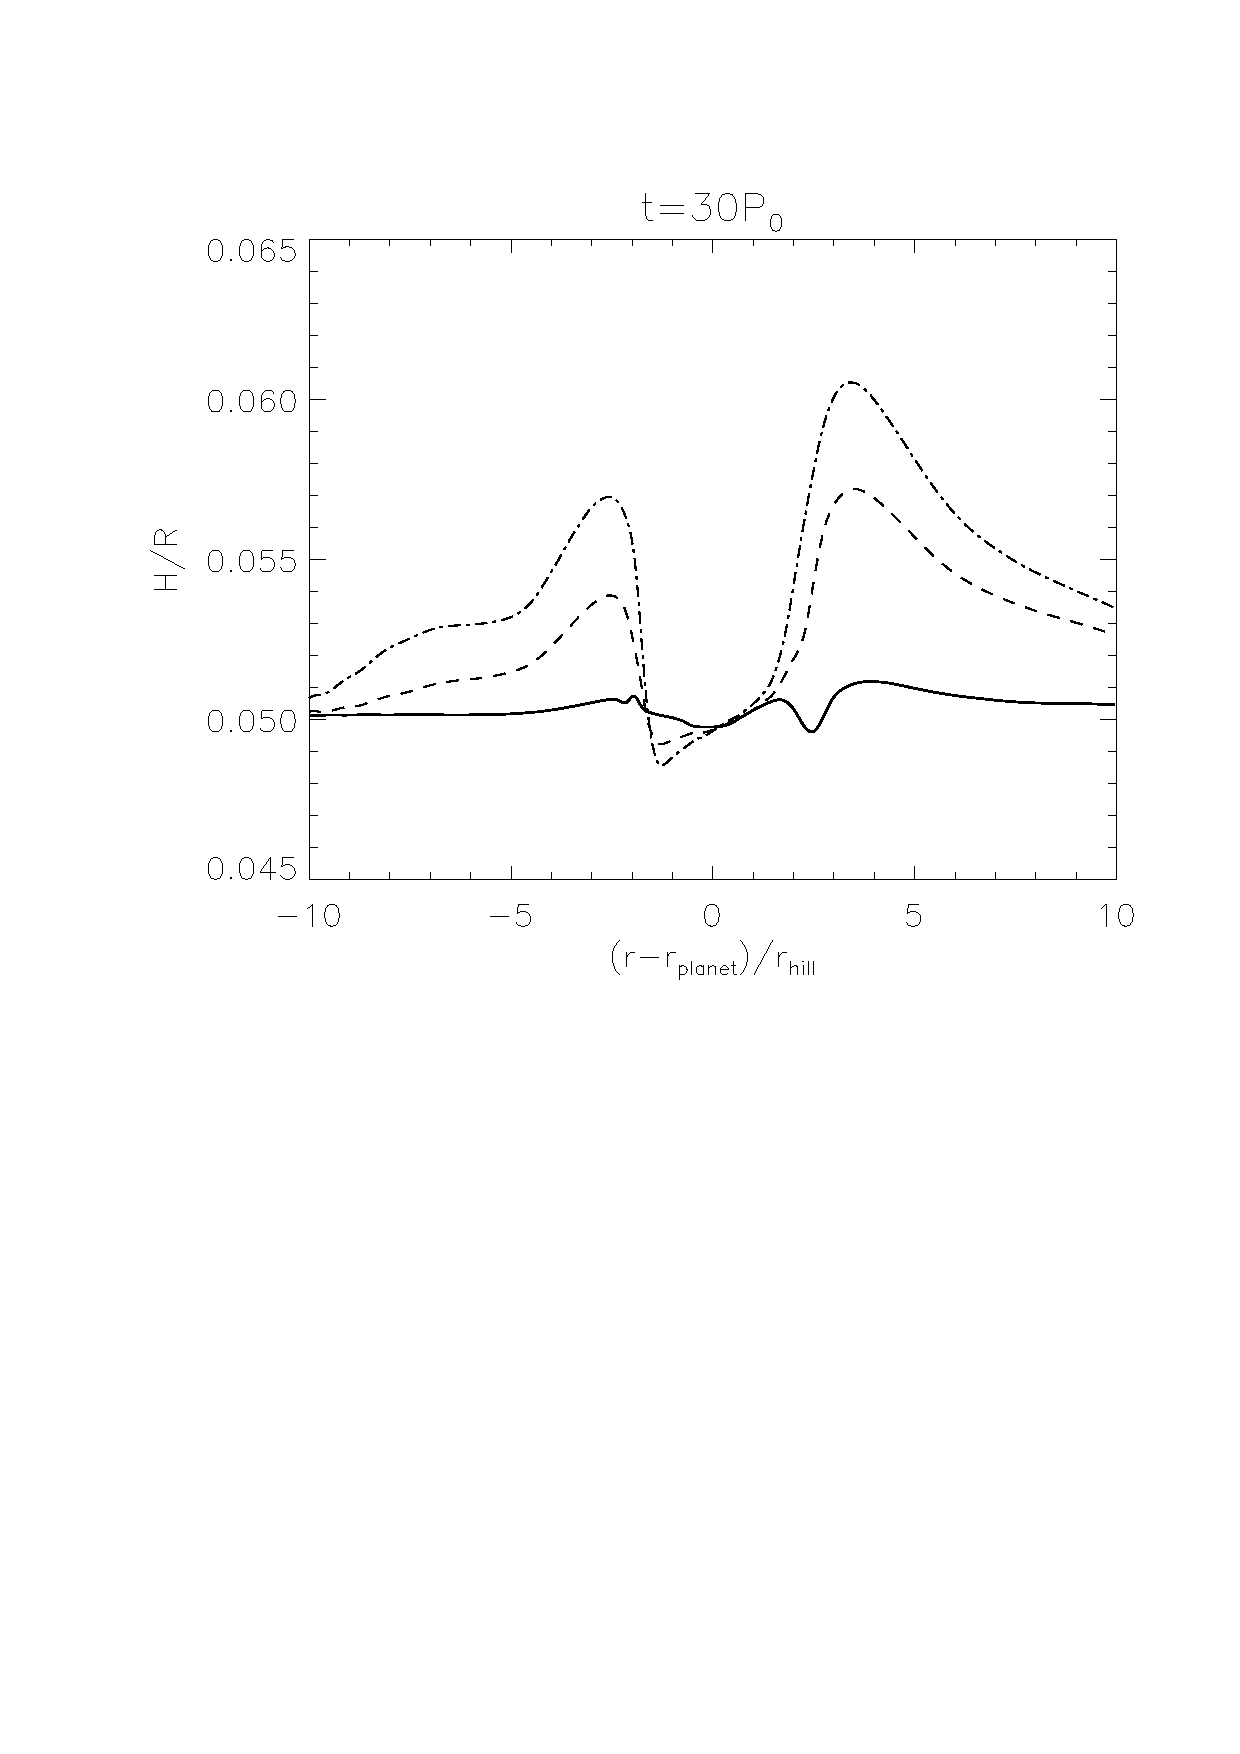
\includegraphics[width=\linewidth,clip=true,trim=0.5cm
    2cm 0cm 1cm]{figures/compare_aspectratio}
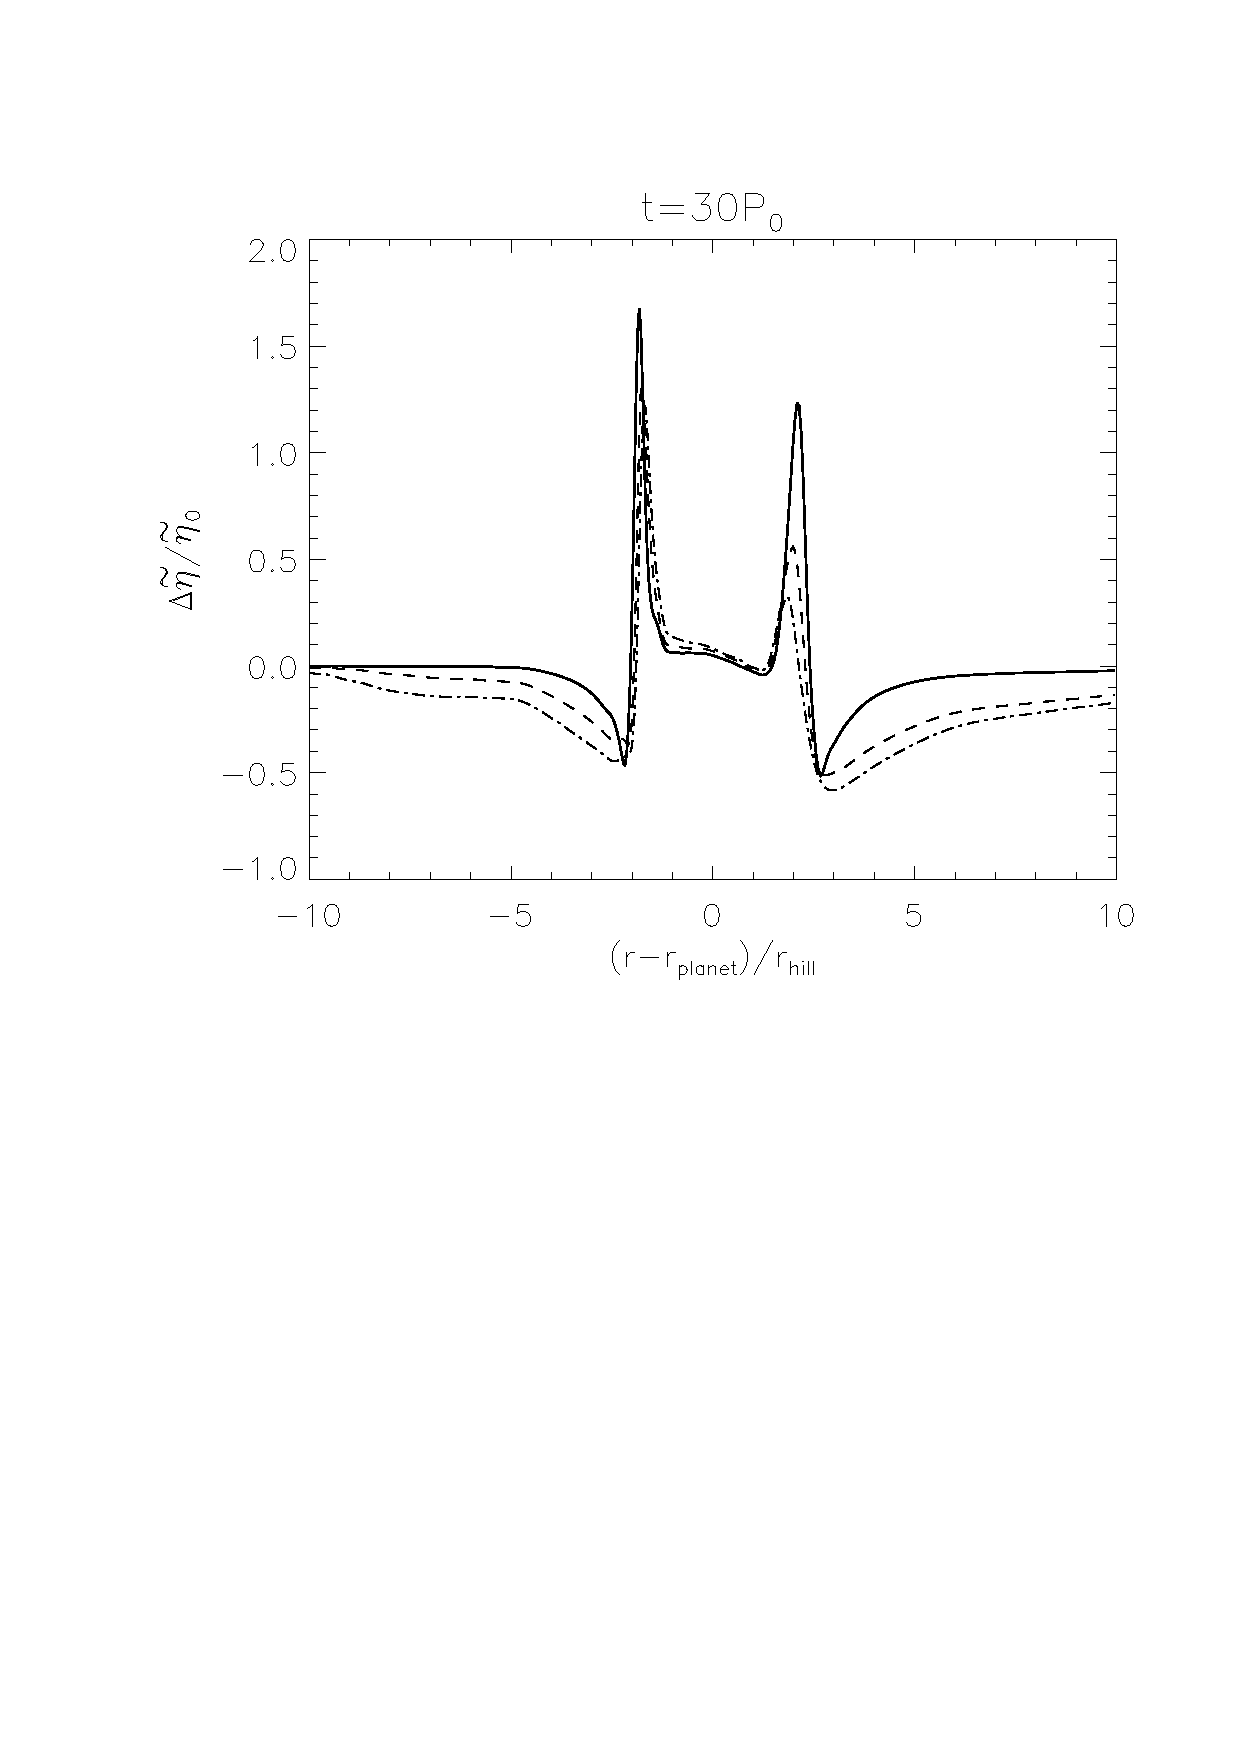
\includegraphics[width=\linewidth,clip=true,trim=0.5cm
    0.5cm 0cm 1cm]{figures/compare_gvortensity}
  \caption{Azimuthally averaged gap profiles at $t=30P_0$ for the
    initial partial gap opened before instability emerges for fast
    (solid, $\tilde{\beta}=0.1$), moderate
    (dashed,  $\tilde{\beta}=1$), and slow cooling (dashed-dot,
    $\tilde{\beta}=10$). The relative surface density 
    perturbation (top), disc aspect ratio (middle) and generalised
    vortensity perturbation (bottom) are shown. \label{intial1D}}  
\end{figure}


%\begin{tabularx}{0.4\textwidth}{l*{10}{R}} \toprule
%  \multicolumn{11}{c}{$\tilde{\beta}=0.1$} \\ \midrule
%  m                    & 1 & 2 & 3 & 4 & 5 & 6 & 7 & 8 & 9 & 10  \\ 
 % $\gamma10^2/\Omega(r_o)$ & 6.56 & 6.82 & 6.73 & 5.78 & 6.00 & 6.38
 % & 5.97 & 5.62 & 4.61 & 3.36   \\ \bottomrule 
%\end{tabularx} 

%\begin{tabularx}{0.4\textwidth}{l*{5}{R}} \toprule
%  \multicolumn{6}{c}{$\tilde{\beta}=1.0$} \\ \midrule
%  m                    & 1 & 2 & 3 & 4 & 5  \\ 
%  $\gamma10^2/\Omega(r_o)$ & 1.27 & 1.28 & 1.35 & 1.01 & 0.61   \\
%  \bottomrule 
%\end{tabularx}

\begin{table}
  \centering
  \caption{Dominant mode and growth rates for
    $\tilde{\beta}=0.1,1.0,10.0$ (fast, moderate, and slow cooling)
    values during `planet-off' simulations \label{modetable}} 
  \hfill
  \begin{minipage}{0.3\linewidth}
    \begin{tabularx}{\textwidth}{l R} 
      \multicolumn{2}{c}{$\tilde{\beta}=0.1$} \\ 
      \toprule
      $m$ & $10^2\sigma/\Omega(r_p)$ \\
      \midrule
      6 & 7.3 \\
      7 & 7.8 \\
      8 & 7.9 \\
      9 & 7.9 \\
      10 & 6.8 \\ 
      \bottomrule
    \end{tabularx}
  \end{minipage}
  \hfill
  \begin{minipage}{0.3\linewidth}
    \begin{tabularx}{\textwidth}{l R} 
      \multicolumn{2}{c}{$\tilde{\beta}=1.0$} \\ 
      \toprule
      $m$ & $10^2\sigma/\Omega(r_p)$ \\
      \midrule
      3 & 2.0 \\
      4 & 2.2 \\
      5 & 2.3 \\
      6 & 1.6 \\
      7 & 1.1 \\ 
      \bottomrule
    \end{tabularx}
  \end{minipage}
  \hfill
  \begin{minipage}{0.3\linewidth}
    \begin{tabularx}{\textwidth}{l R} 
      \multicolumn{2}{c}{$\tilde{\beta}=10.0$} \\ 
      \toprule
      $m$ & $10^2\sigma/\Omega(r_p)$ \\
      \midrule
      1 & 1.1 \\
      2 & 1.6 \\
      3 & 1.7 \\
      4 & 1.2 \\
      5 & 0.1 \\ 
      \bottomrule
    \end{tabularx}
  \end{minipage}
  \hfill
\end{table}

\subsection{Axisymmetric stability}
The initial planet-disc interaction form bumps and grooves in the gap profiles
which can potentially be unstable due to axisymmetric instabilities. The
generalised local axisymmetric stability condition is the Solberg-Hoiland
criterion,  
\begin{align}
  \kappa^2+N^2 \geq 0 
\end{align}
where
\begin{align}
 N^2=\frac{1}{\Sigma} \frac{\partial P}{\partial r}
 \left(\frac{1}{\Sigma} \frac{\partial \Sigma}{\partial
     r}-\frac{1}{\gamma P} \frac{\partial P}{\partial r}  \right) 
\end{align}
is the square of the Brunt-V\"ais\"al\"a frequency. 
At the outer gap edge $r=r_p+2.5r_h$,  where the RWI is excited
(see below),{\bf  we find $\kappa^2 + N^2$ reaches local minimum with a value
$\sim 0.45 \, \Omega^2(r_p)$
%$\sim 2\times10^{-4}$ (code units)
 for all $\tilde\beta$. The
Brunt-V\"ais\"al\"a frequency at the outer gap edge is
$N\sim 10^{-2} \, \Omega^2(r_p)$,}
% $N\sim 10^{-5}$,
decreasing marginally with longer cooling rate. 
The Solberg-Hoiland criteria is similarly satisfied for the entire 2D disc throughout the 
simulations.
Thus for all values of $\tilde\beta$ the planet-induced gaps are
stable to axisymmertic instabilities. 

% {\bf Brunt frequency the same for all cooling?:small decrease with beta,
%  not more than order of magnitude}

%  {\bf i assume this means the azimuthally averaged
%   values. do you ever get $N^2<0$ anywhere in the 2D disc?:
%  This was not for azimuthal average, below 0 inside gap but kappa+N always above 0 everywhere} 

\subsection{Non-axisymmetric instability}\label{linear}
We now examine the evolution of the gap for $t>30P_0$, with the
planet potential switched off, but with an added surface density
perturbation. For all three cooling times $\tilde{\beta}=0.1,\, 1.0,\,
10$, we observe exponential growth of non-axisymmetric
structures. An example is shown in Fig. \ref{linearmodes} for 
$\tilde{\beta}=10$. We characterise these
modes with an azimuthal wavenumber $m$ and growth rate $\sigma(m)$ as defined by
Eq.~\ref{fouriertransform}---\ref{growth}. Mode amplitudes were
averaged over $r-r_p\in[2,5]r_h$. Table \ref{modetable}
lists the growth rates measured during 
linear growth for 5 values of $m$ centred around that with maximum
growth rate. 

\begin{figure}
  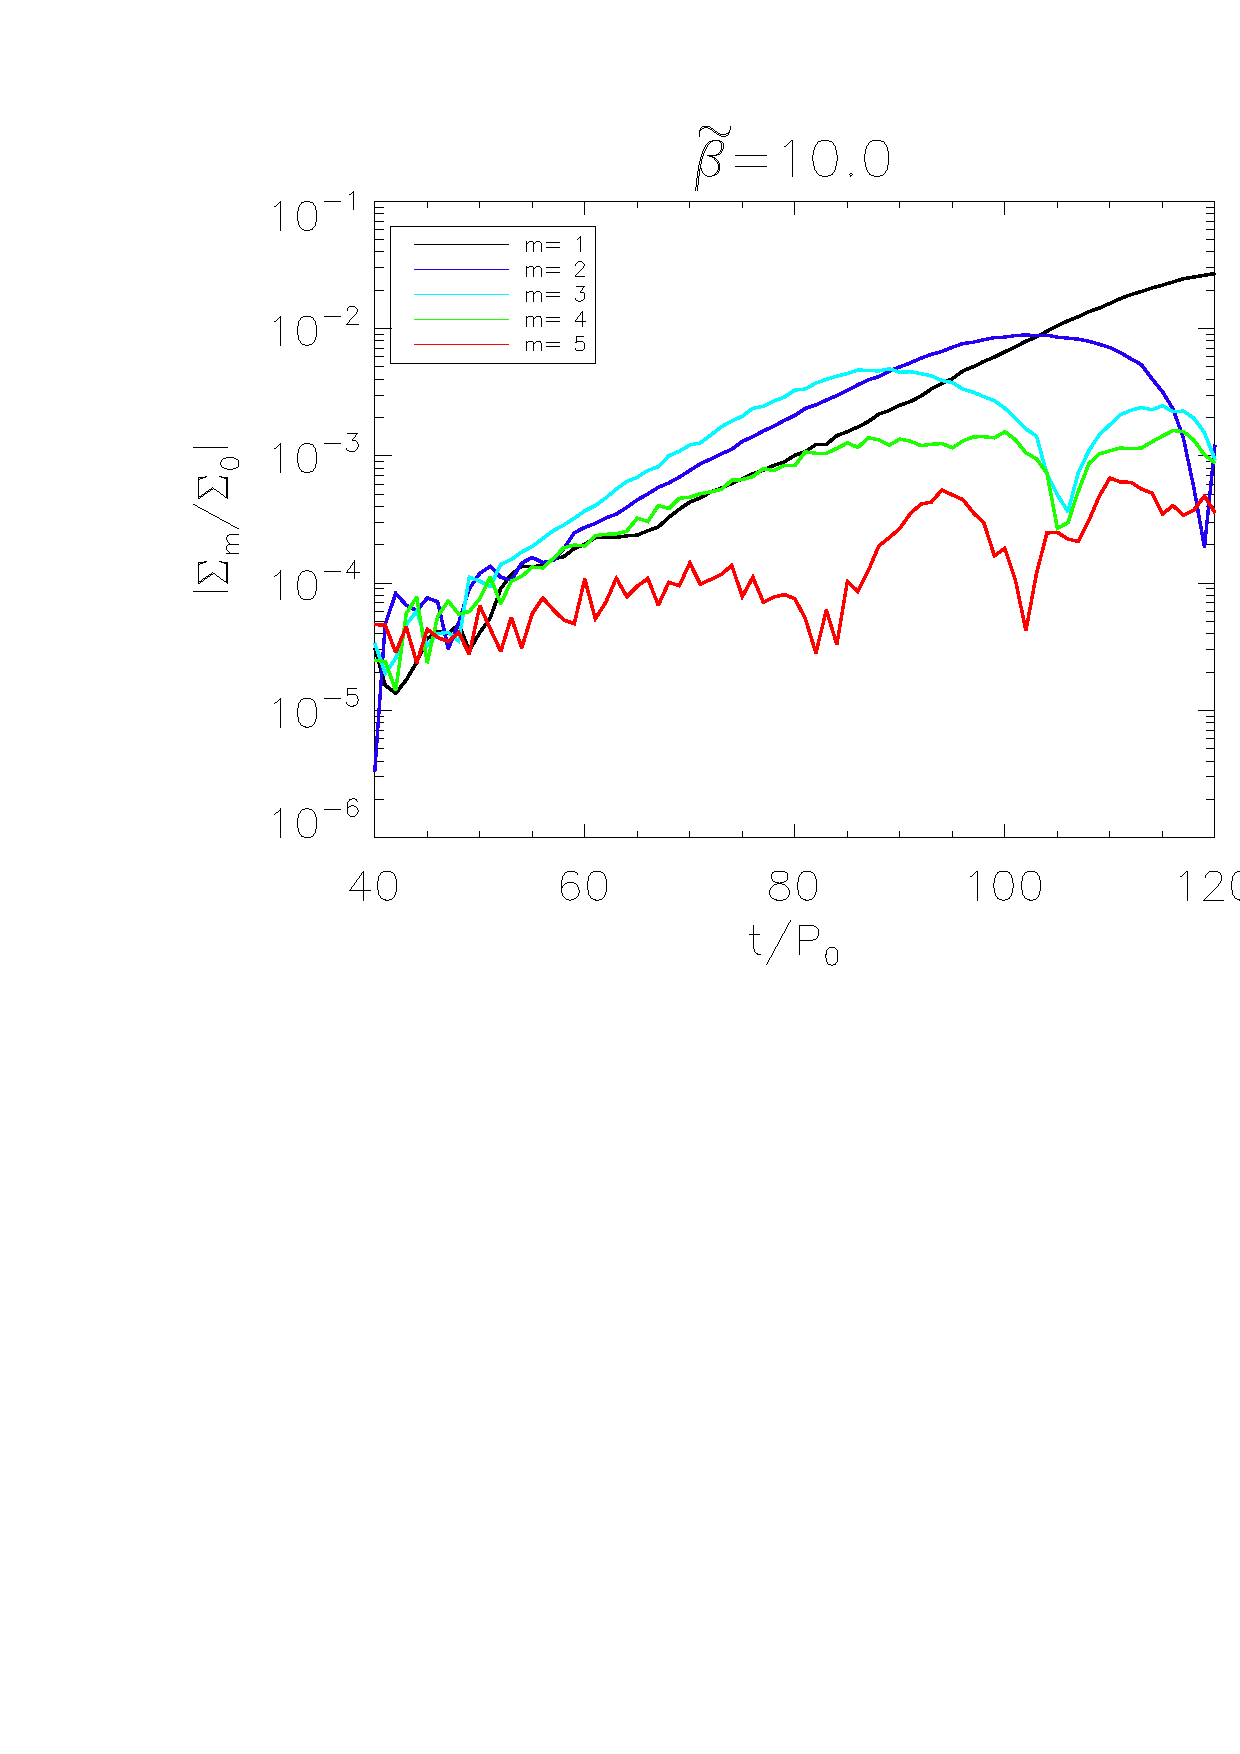
\includegraphics[width=\linewidth,clip=true,trim=1.2cm
  0cm 0cm 0cm]{figures/linear_stability}
  \caption{Evolution of azimuthal Fourier modes of disc surface
    density, non-dimenionlised by the initial axisymmetric component 
    $\Sigma_0(t=0)$, for the
    `planet-off' simulation with $\tilde{\beta}=10$. Colours correspond
    to different $m$ values. The $m=3$ component is the fastest growing
    mode during linear growth with a growth rate of 
    $\gamma=0.017\Omega(r_p)$.\label{linearmodes}}
  % {\bf is the $\Sigma_0$ at t=0?} }  
\end{figure}

%%%%%%%%%%%%%%%%%%%%%%%%%%%%%%%%%%%%%%%%%%%%%%%%%%%%%%%%%%%%%%%%%%%%%%%

Table \ref{modetable} show that as
$\tilde{\beta}$ is increased from $ 0.1\rightarrow10$ the dominant
azimuthal Fourier mode decreases from $ m=9\rightarrow3$ and the
respective growth rate decreases from $ \gamma/\Omega(r_p)=0.079
\rightarrow 0.017$. However, despite two orders of magnitude increase in the
cooling time, the instability remains dynamical with characteristic  growth time
$\lesssim 10P_0$. Snapshots of the instability in for  
the different $\tilde\beta$ are shown in Fig \ref{2Dlinear}. 

{\bf We also simulated a locally isothermal disk where the sound-speed is
  held fixed, which yield a most unstable growth rate
  $\sigma/Omega(r_p)\simeq 0.05$, compared with a value of $0.08$ for
  a case with $\tilde{\beta}=0.01$.}   
%Isothermal simulations with set sound speed where also analyzed
%  showing growth rates $\sim 5 \times 10^{-2} / \Omega(r_p)$. }
%In comparison nearly isothermal simulation with $\tilde\beta=0.01$ had growth rates $\sim 8\times 10^52 / \Omega(r_p)$}

These `planet-off' simulations show that gap edges become more stable with
longer cooling times. This is expected because larger $\tilde{\beta}$
results in hotter gap profiles at $t=30P_0$ with less pronounced
generalised vortensity minima. Stabilisation with increased
cooling time is therefore due to a smoother basic state for the
instability, as it is more difficult for the planet to open a gap if
the disc is allowed to heat up. 

\begin{figure}
  \centering
  \subfigure{
    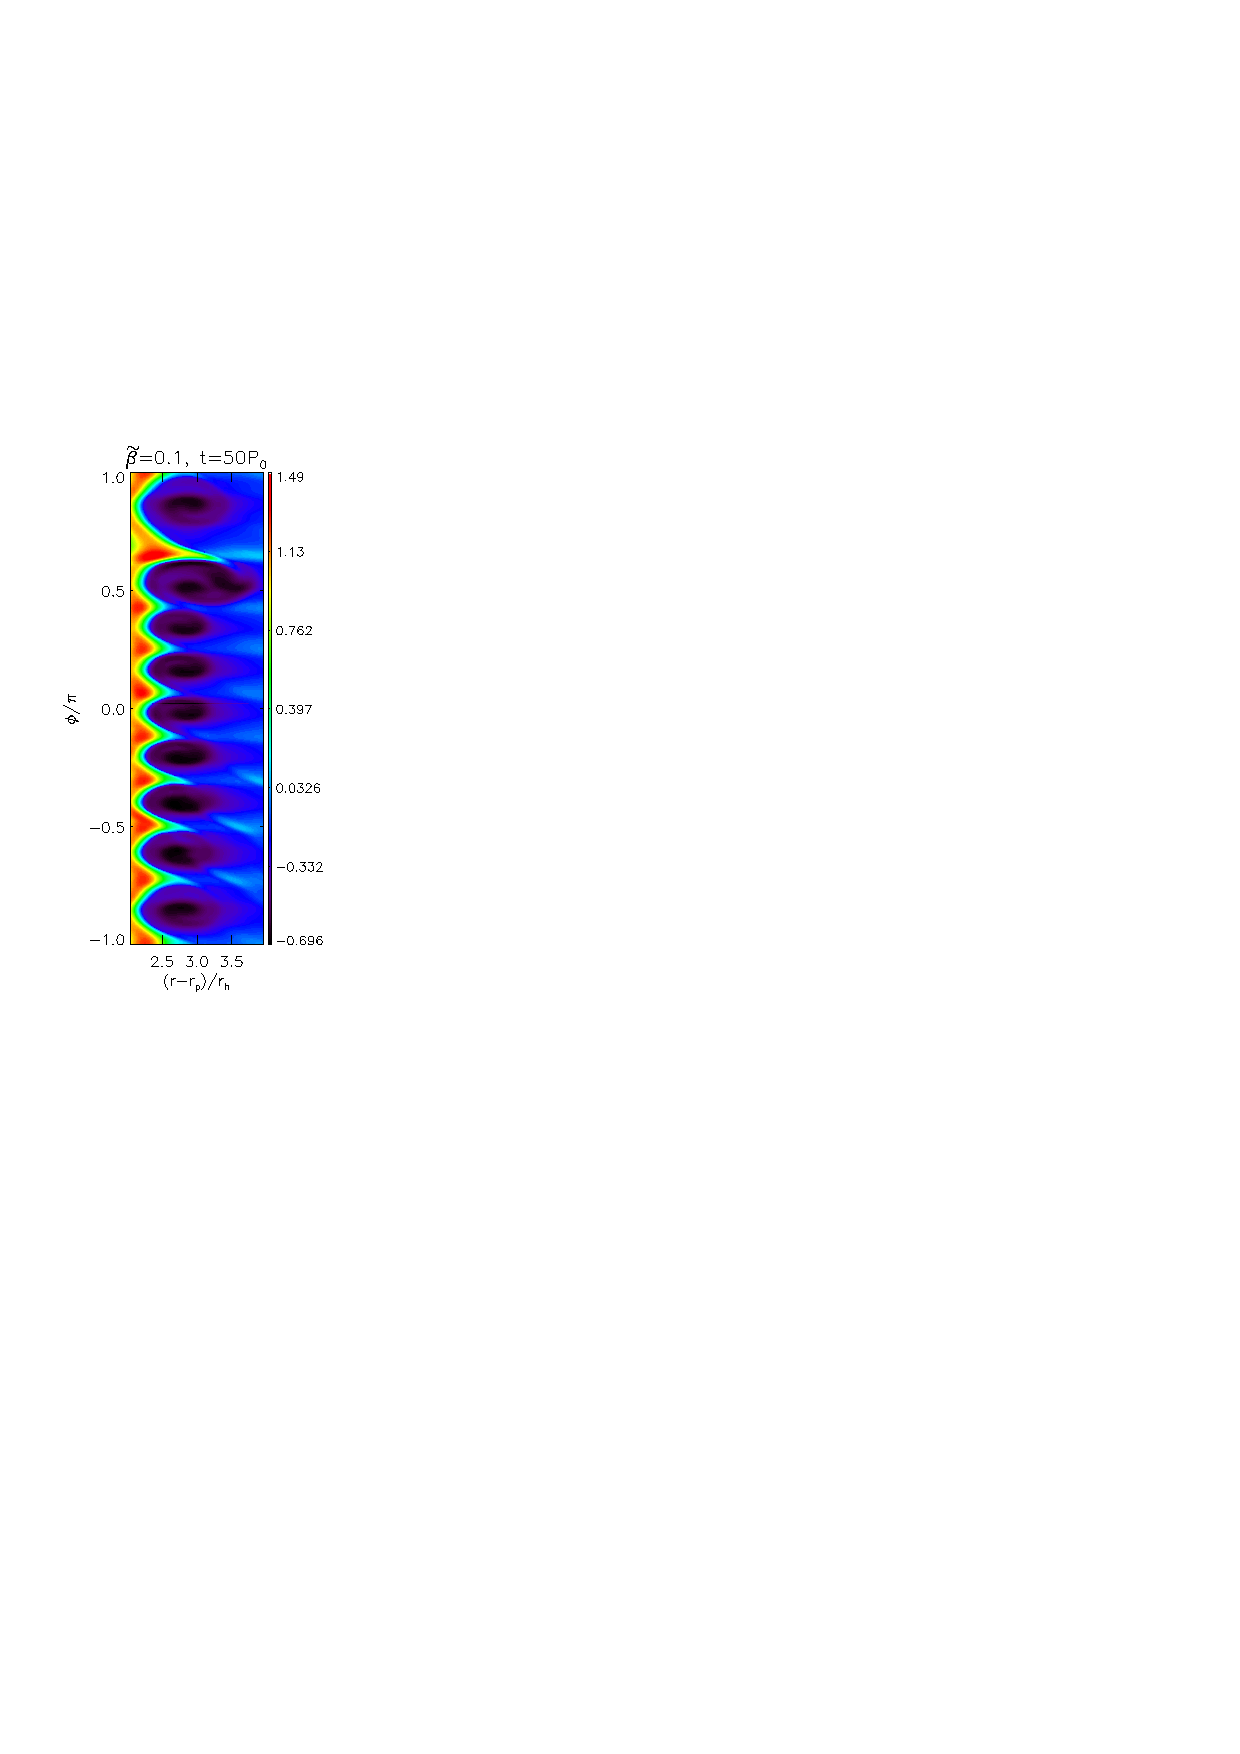
\includegraphics[width=0.3\linewidth]{figures/analysis_gvortensity50}
  }
\hfill
  \subfigure{
    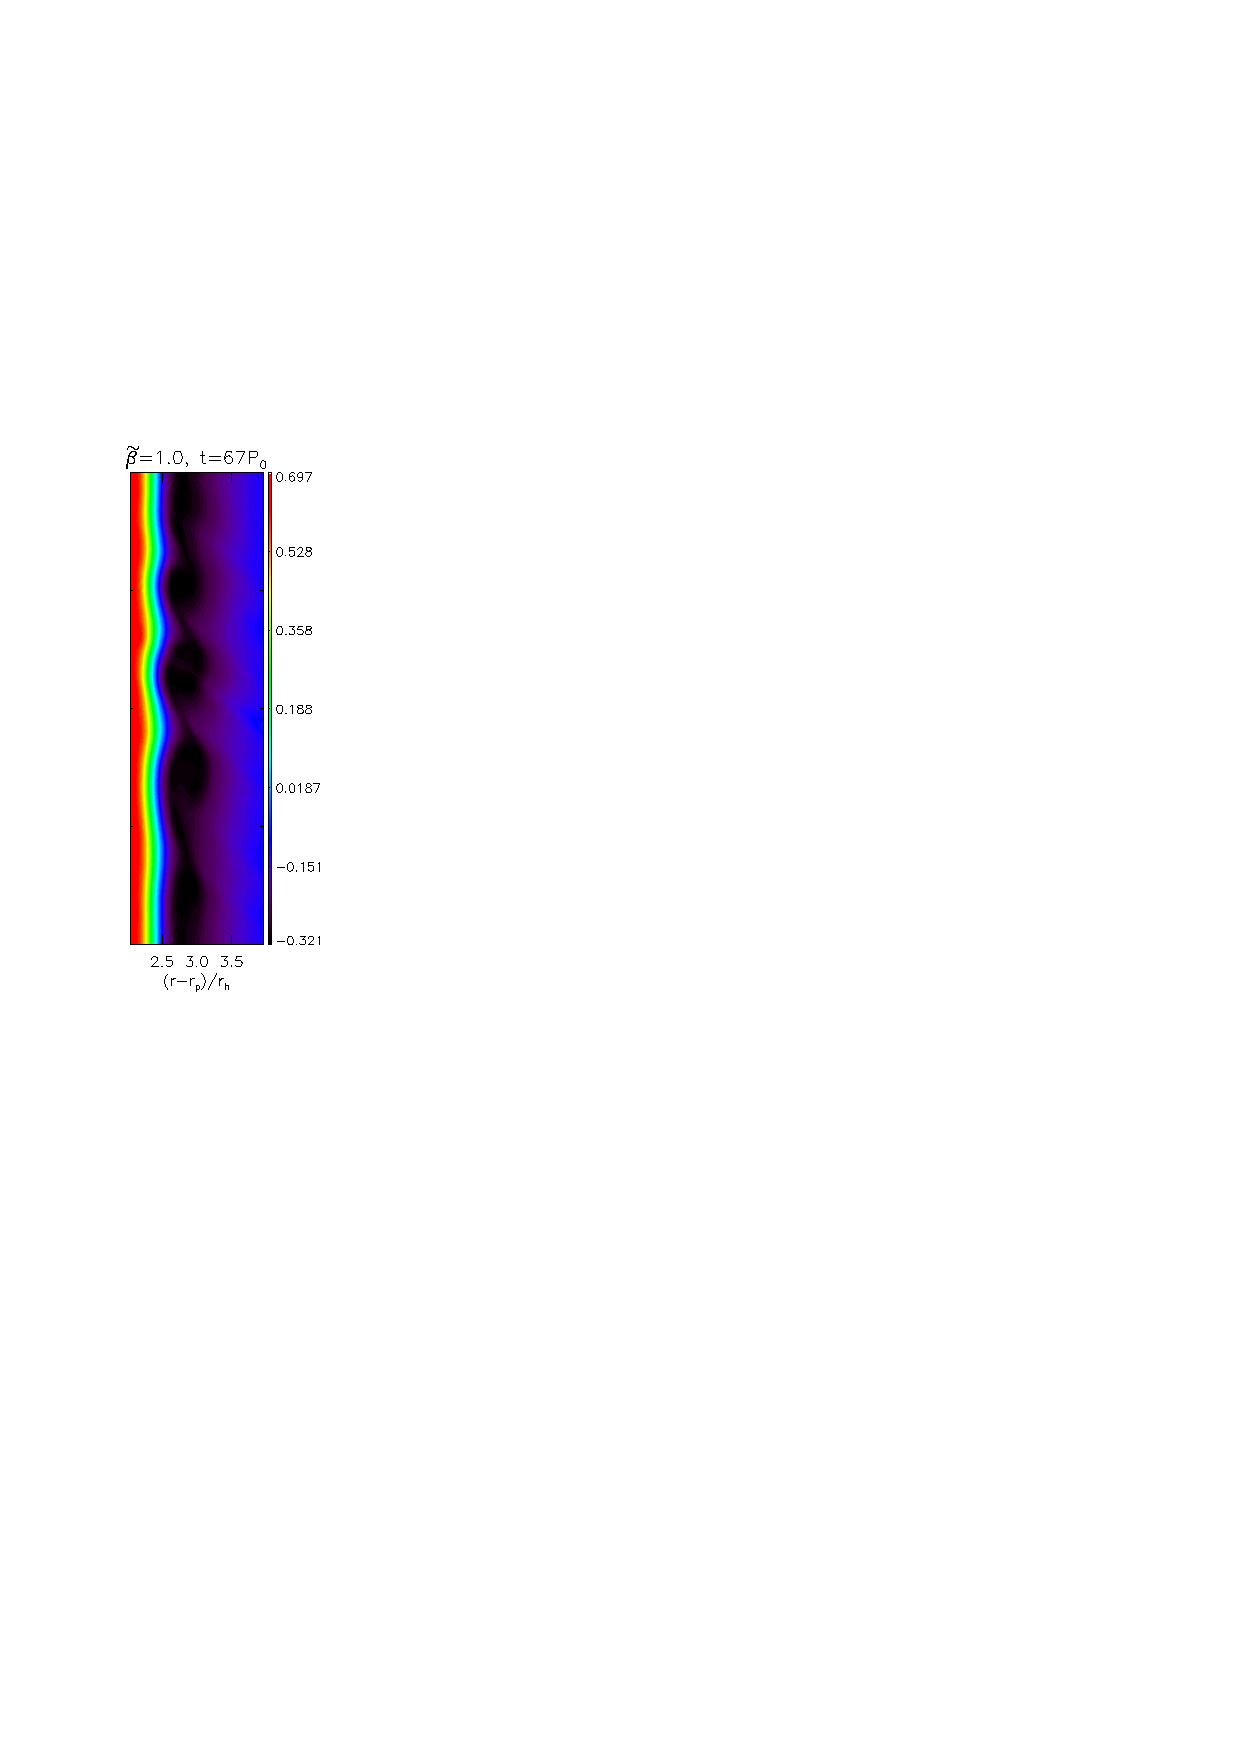
\includegraphics[width=0.3\linewidth]{figures/analysis_gvortensity67}
  }
\hfill
  \subfigure{
    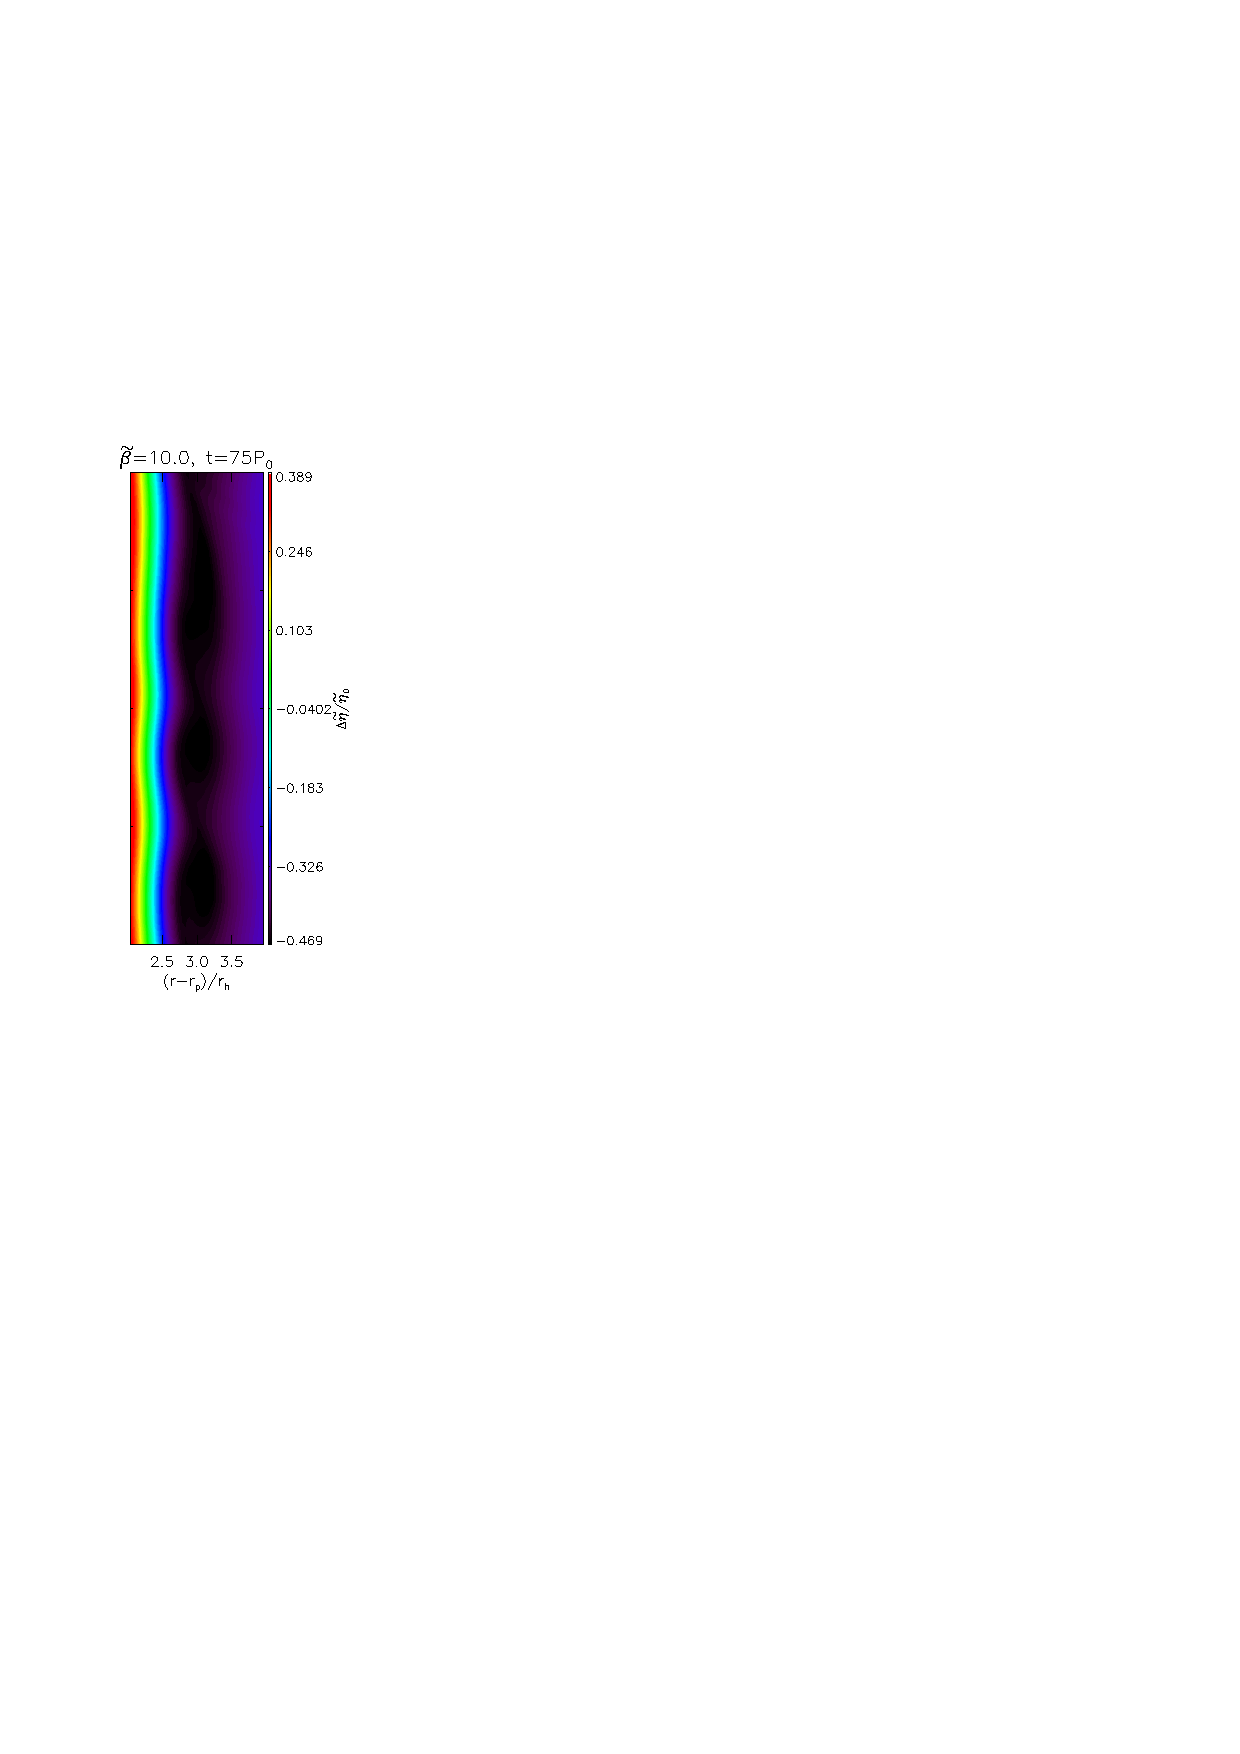
\includegraphics[width=0.3\linewidth]{figures/analysis_gvortensity75}
  }  
  \caption{Generalised vortensity perturbation (relative to $t=0$) for
    cases of $\tilde{\beta}=0.1,1,10$ (left,middle,right) during
    the growth of non-axisymmetric modes. The planet potential has
    been switched off.  The number of vortices
    decrease as $\tilde{\beta}$ increases. Note that snapshots are
    taken later for increasing $\tilde{\beta}$ because it takes longer
    for the vortices to grow and become visible with increasing cooling time. 
    \label{2Dlinear} 
  } 
\end{figure}

\subsubsection{Nearly adiabatic discs}
\label{adiabatic_section}

The above `planet-off' simulations are not formally linear
stability calculations, because the cooling time is comparable or shorter
than the instability growth time, $t_c\lesssim\gamma^{-1}$.  
Thus the disk cools back to its initial temperature corresponding to
$h=0.05$ before or during the instability growth, so we do not 
have a steady basic state to formulate a standard linear stability 
problem. 

In order to capture the effect of a heated gap edge, we ran a simulation with 
$\tilde{\beta}=100$, corresponding to an almost adiabatic disc.  
In this simulation the cooling rate is slow enough that the gap 
temperature profile (e.g. middle panel of Fig. \ref{intial1D}) changes
only marginally over the instability growth timescale. 

We find very similar gap profiles and mode growth rates for
$\tilde{\beta}=100$ as with $\tilde{\beta}=10$. At $t=30P_0$, the disc only heats up to
values $h\simeq0.06$ in the nearly adiabatic case. This is close to
the original temperature of $h=0.05$, so linear growth rates are not expected
to change significantly \citep{li00}. 

According to \cite{li00}, increasing $h$ increases linear growth rates
of the RWI because it is pressure-driven. However, in the case 
of disc-planet interaction, increasing $h$ has a stabilizing effect
through the setting up the gap profile because it results in smoother gap
edges. The fact that we observe smaller growth rates as $h$ is
increased indicates that for planetary gaps, the importance of $h$ on
the \emph{linear} RWI is through setting up the gap profile, i.e. basic
state for the instability (as opposed to the linear response). 

\subsection{Long term evolution} \label{nonlinearplanetoff} 
% {\bf typical rossby numbers for these `planet-off' vortices? do
%   stronger vortices (beta=0.1) dissipate faster?:very complicated
% maybe not worth discussing since just comparison to planet-off}

We also extended these `planet-off' simulations into the non-linear
regime. After the linear growth phase of the vortices, vortex merging
takes hold on timescales of up to $150P_0$, until there is one vortex
left. We find the vortex merging
time is dependent on the growth rates of the modes and saturation
timescales, with the slowest growing modes in $\tilde\beta=10$ taking
the longest to merge.  

Fig.\ref{planetofflifetimeplot} shows evolution of the $m=1$ surface
density component, which represents the amplitude of the post-merger
single vortex. For completeness we also ran intermediate cases with
$\tilde{\beta}=0.5$ and $5.0$. The amplitude of the initially formed vortex was 
found to decrease with increased cooling rate. The vortices simply decay on a
timescale of $O(10^3)$ orbits with faster decay for stronger vortices
(which are obtained with faster cooling rates). {\bf This decay is 
  probably due to numerical viscosity. During the slow decay the
  vortex elongates (weakens) while its radial width remains $O(H)$, so
  its surface density decreases. (true?)} 
We will see in the
next section that this behaviour {\bf after linear growth} is very
different to when the planet potential is kept on. 

%Interestingly, though, vortices arising from the stronger
%instabilities (shorter cooling times or lower $\tilde{\beta}$) decays
%faster.   

%main point: no planet: only get growth during linear instability
%           with palnet: further growth after linear regime

\begin{figure}
  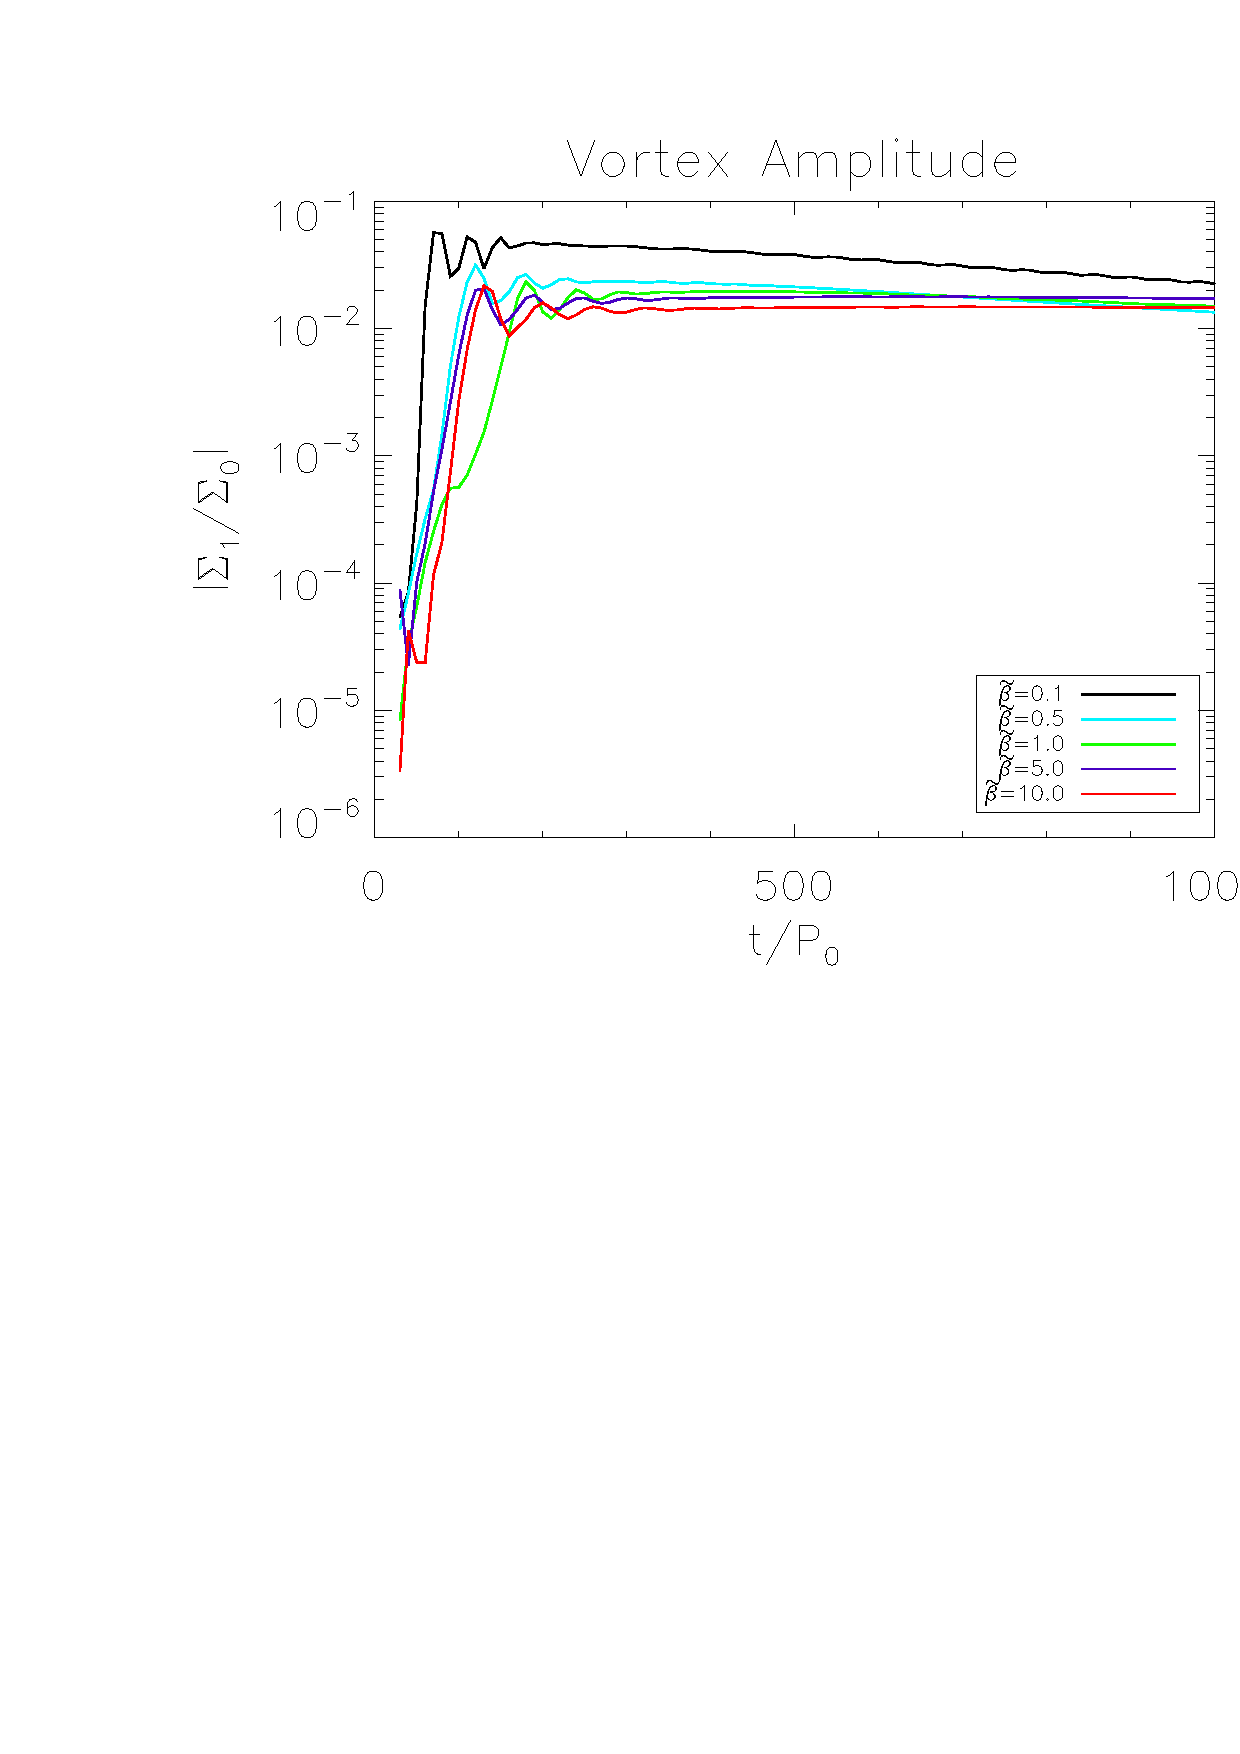
\includegraphics[width=\linewidth,clip=true,trim=0.5cm
  0cm 0cm 1.1cm]{figures/longterm_planetoff}
  \caption{Long term simulations without the planet potential after
    the gap is set up. The $m=1$ surface density component,
    non-dimenionlised by the initial $m=0$ component, at the
    outer gap edge is shown as a function of the cooling timescale. 
  } \label{planetofflifetimeplot}
\end{figure}

%%%%%%%%%%%%%%%%%%%%%%%%%%%%%%%%%%%%%%%%%%%%%%%%%%%%%%%%%%%%%%%%%%%%%

\section{Non-linear evolution of
  gap-edge vortices with finite cooling time}\label{nonlinear} 
We now examine long-term simulations of gap-edge vortices for
$\tilde{\beta}=0.1,0.5,1,5,10$. The planet potential is kept on
throughout. We employ a grid with $(N_r,N_{\phi})=(512,1024)$ in order
for these 
simulations to be computationally feasible. We also use a larger
disc with $r_{\mathrm{out}}=45r_{\mathrm{in}}$ to minimise boundary
effects on vortex evolution, and apply open boundaries at
$r=r_\mathrm{in},\,r_\mathrm{out}$. We comment that lower-resolution
simulations with $(N_r,N_{\phi})=(256,512)$ were initially carried
out, which show similar behaviour and trends as the high-resolution
runs reported below.   

\subsection{Generic evolution} 
The linear growth of the RWI and vortex-formation is followed by 
vortex merging. We now find merging timescales independent of
$\tilde\beta$, and by $60P_o$ only one vortex remains. 
The evolution of the amplitude of the $m=1$ surface density component,
averaged over $r-r_p\in[2,10]r_h$, is shown in Fig.~\ref{lifetimeplot} 
for different $\tilde\beta$. The initial, post-merger vortex amplitude
is found to be weaker for longer cooling rates (which have smaller 
linear growth rates). 

\begin{figure}
  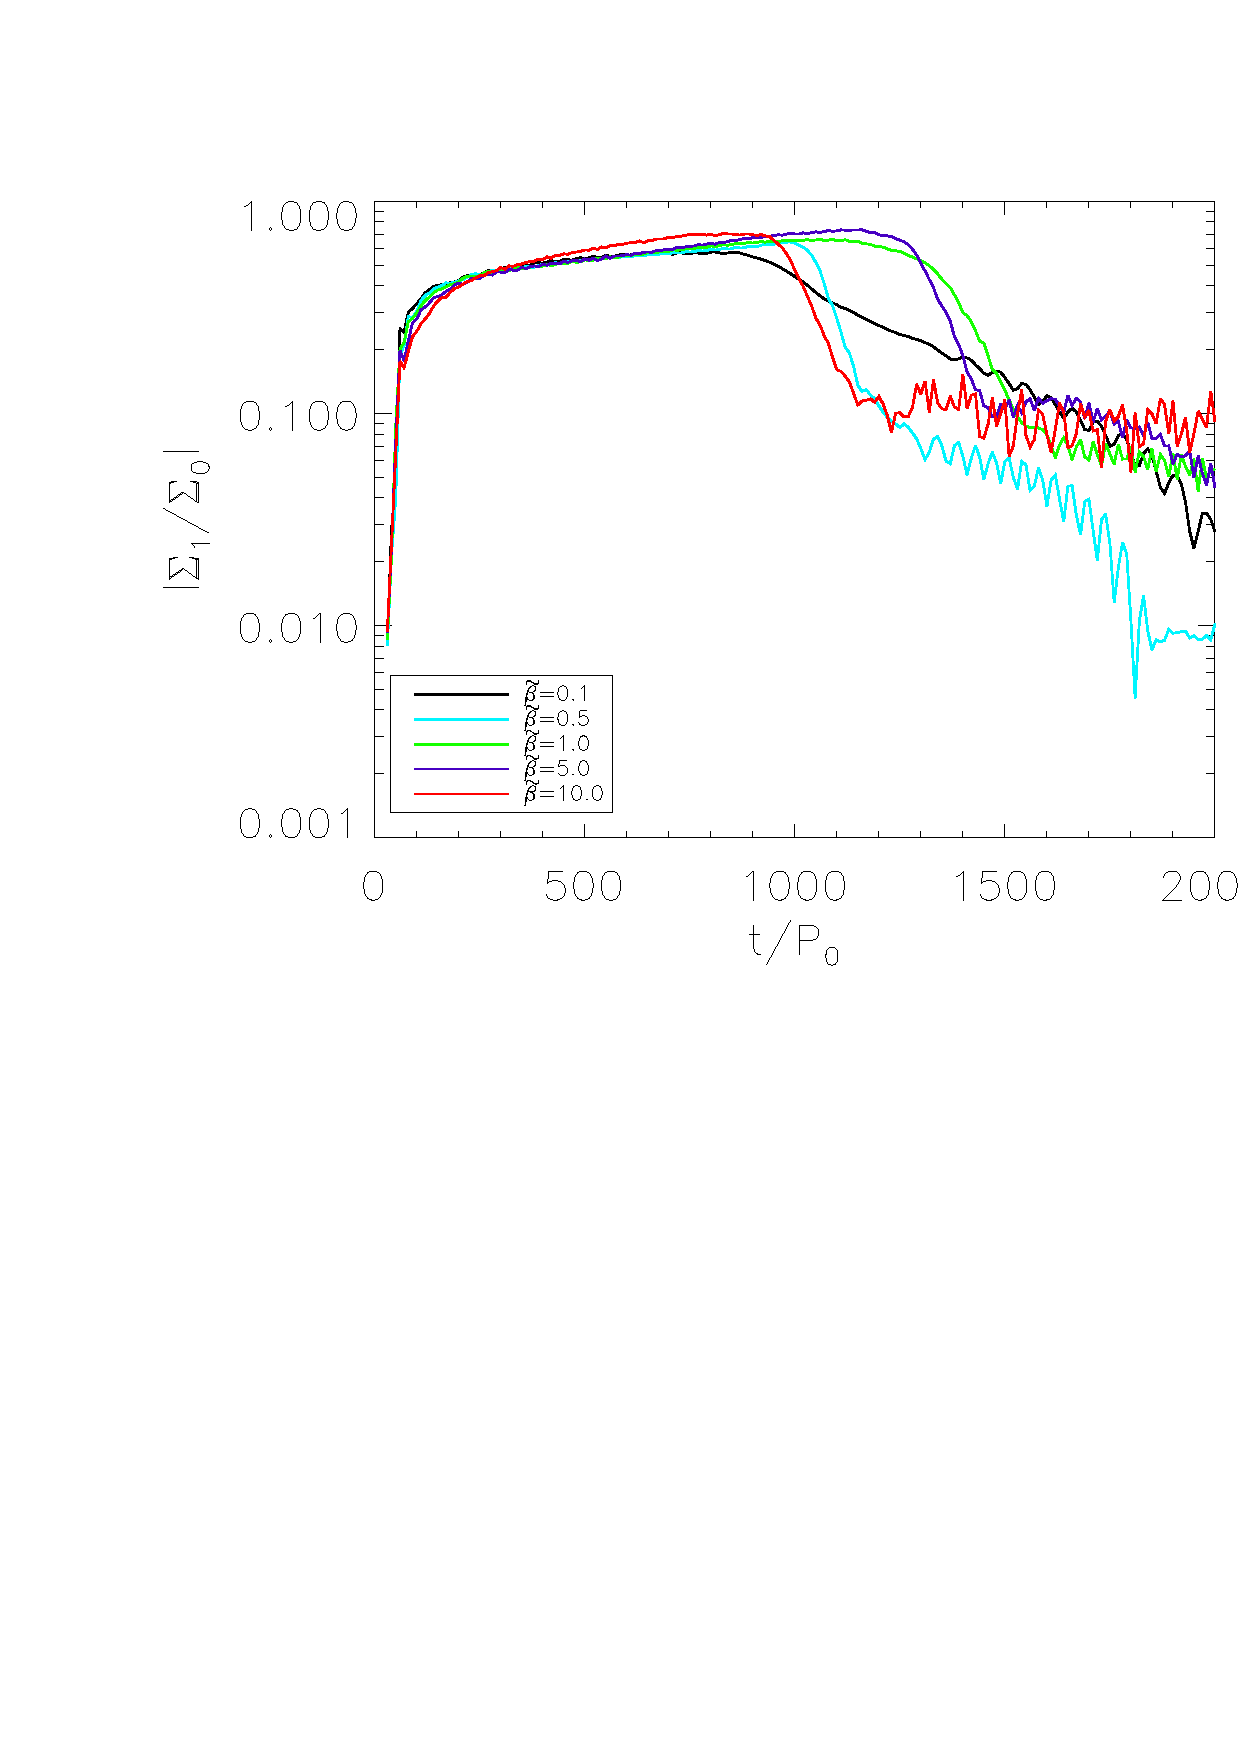
\includegraphics[width=\linewidth,clip=true,trim=0.5cm
  0cm 0cm 1cm]{figures/longterm_stability}
  \caption{Evolution of the non-dimesnionalized $m=1$ surface density component
    for long term
    simulations with the planet potential kept on. Notice there is
    vortex growth after the initial linear growth, which
    contrasts to Fig. \ref{planetofflifetimeplot}, where vortices
    decay in the absence of continuous disc-planet interaction. 
    \label{lifetimeplot}}   
\end{figure}

In all cases the system remains in a quasi-steady state for
$\gtrsim800P_0$ with a single vortex circulating 
the outer gap edge at the local Keplerian  
frequency. 
Fig. \ref{Vortex2D} shows a typical plot of the relative 
surface density perturbation in this state. During this stage, the 
vortex intensifies. This is better shown in Fig. \ref{rossbyplot} as the
evolution of Rossby numbers measured at the vortex centres.  
%As the vortex forms it has an initial 
%Rossby number $Ro\approx-0.1$ for all $\tilde\beta$
%(implying anti-cyclonic 
%motion). 
The Rossby number increases in magnitude during quasi-steady state,
but the maximum $|Ro|$ is similar for all $\tilde{\beta}$: the vortex
reaches a characteristic value of $Ro\approx-0.35$ for 
$\tilde\beta=0.1$ and $Ro\approx -0.45$ for $\tilde\beta=10$.    

% {\bf Maybe useful to have a Rossby number v.s. time plot to complement
% mode amplitude plot. }

\begin{figure}
  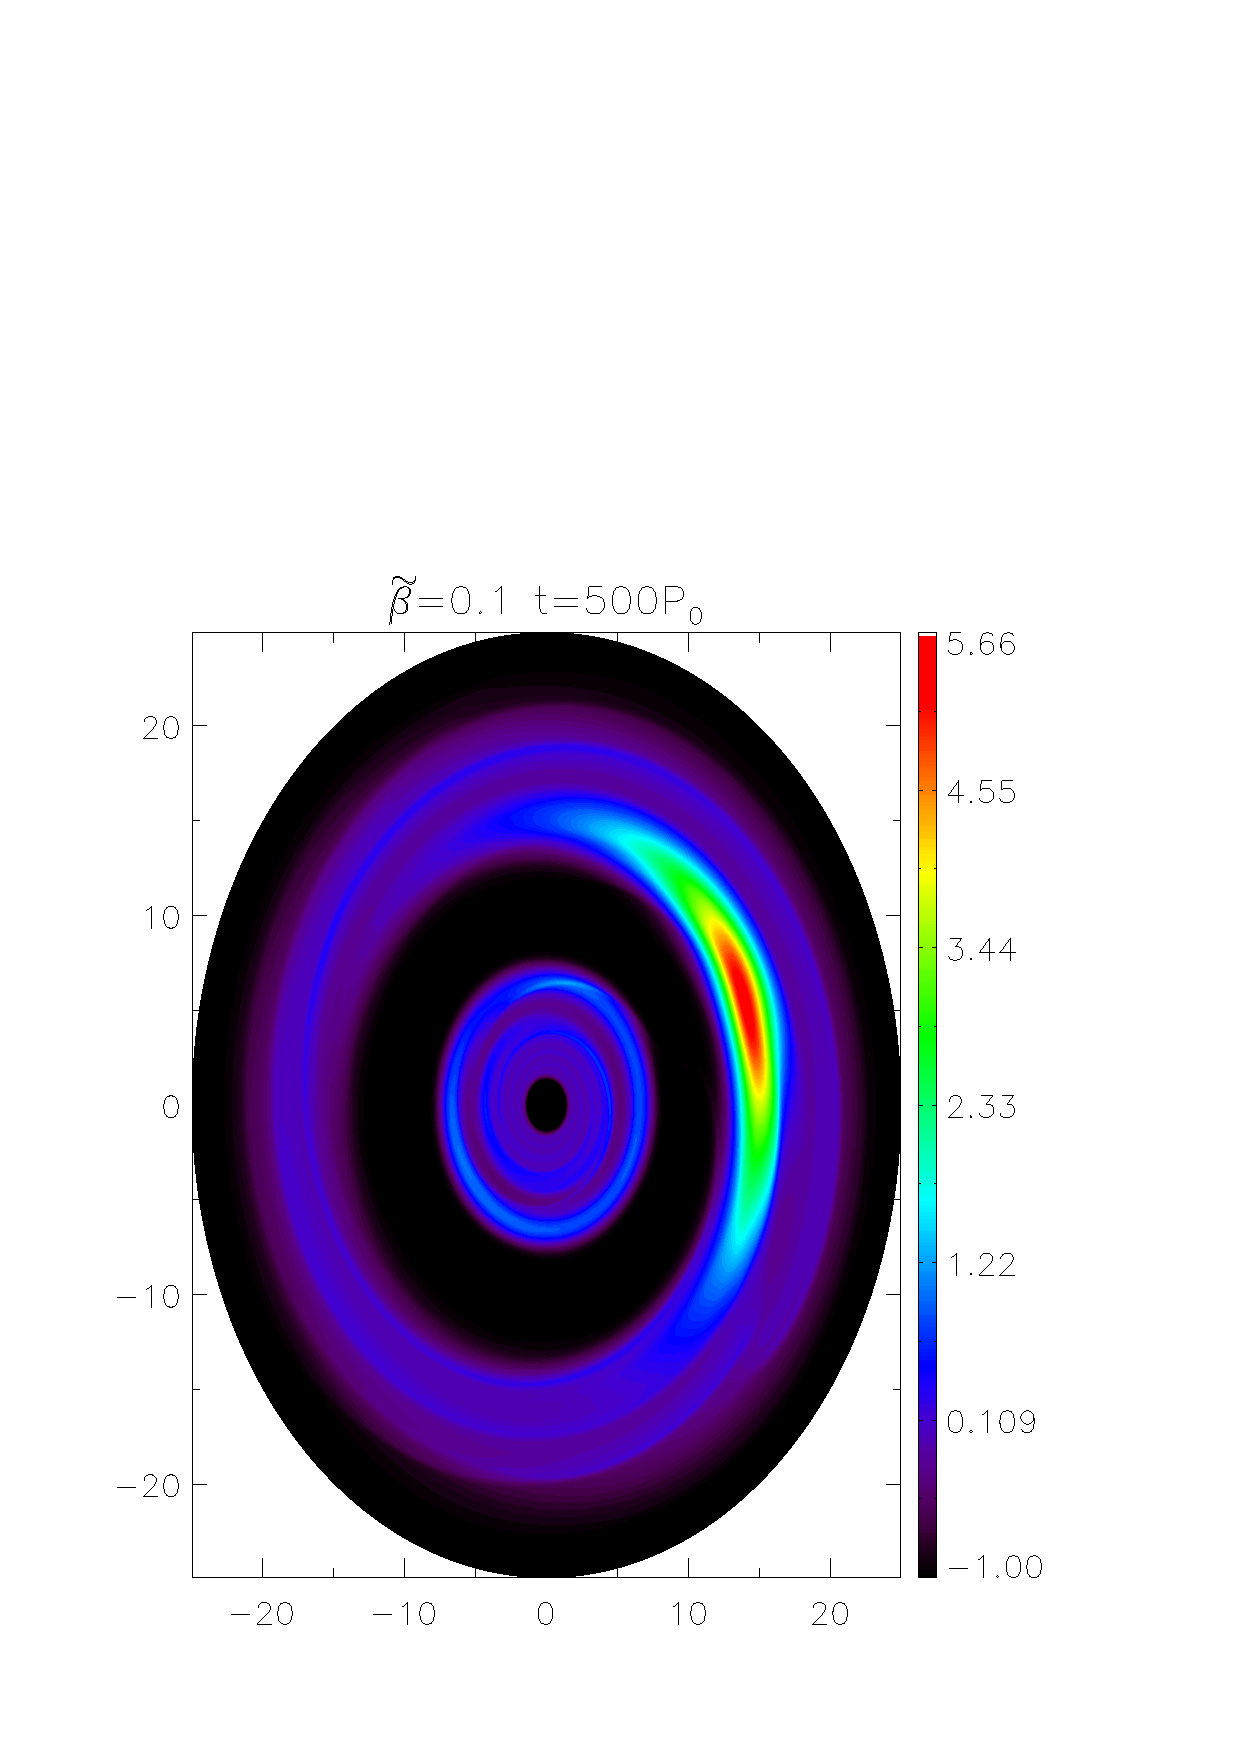
\includegraphics[width=\linewidth,height=\linewidth]{figures/vortex2D}
  \caption{Relative surface density perturbation for the
    $\tilde\beta=0.1$ case during quasi-steady state with a single
    vortex at the outer gap edge. The plot for other values of the cooling time
    $\tilde{\beta}$ are similar. {\bf The decrease in the surface
      density near} $r\sim 40 r_\mathrm{in}$ {\bf arises from mass loss due to the open
      boundary condition imposed at} $r_\mathrm{out}$.
    \label{Vortex2D} }
\end{figure}



\begin{figure}
  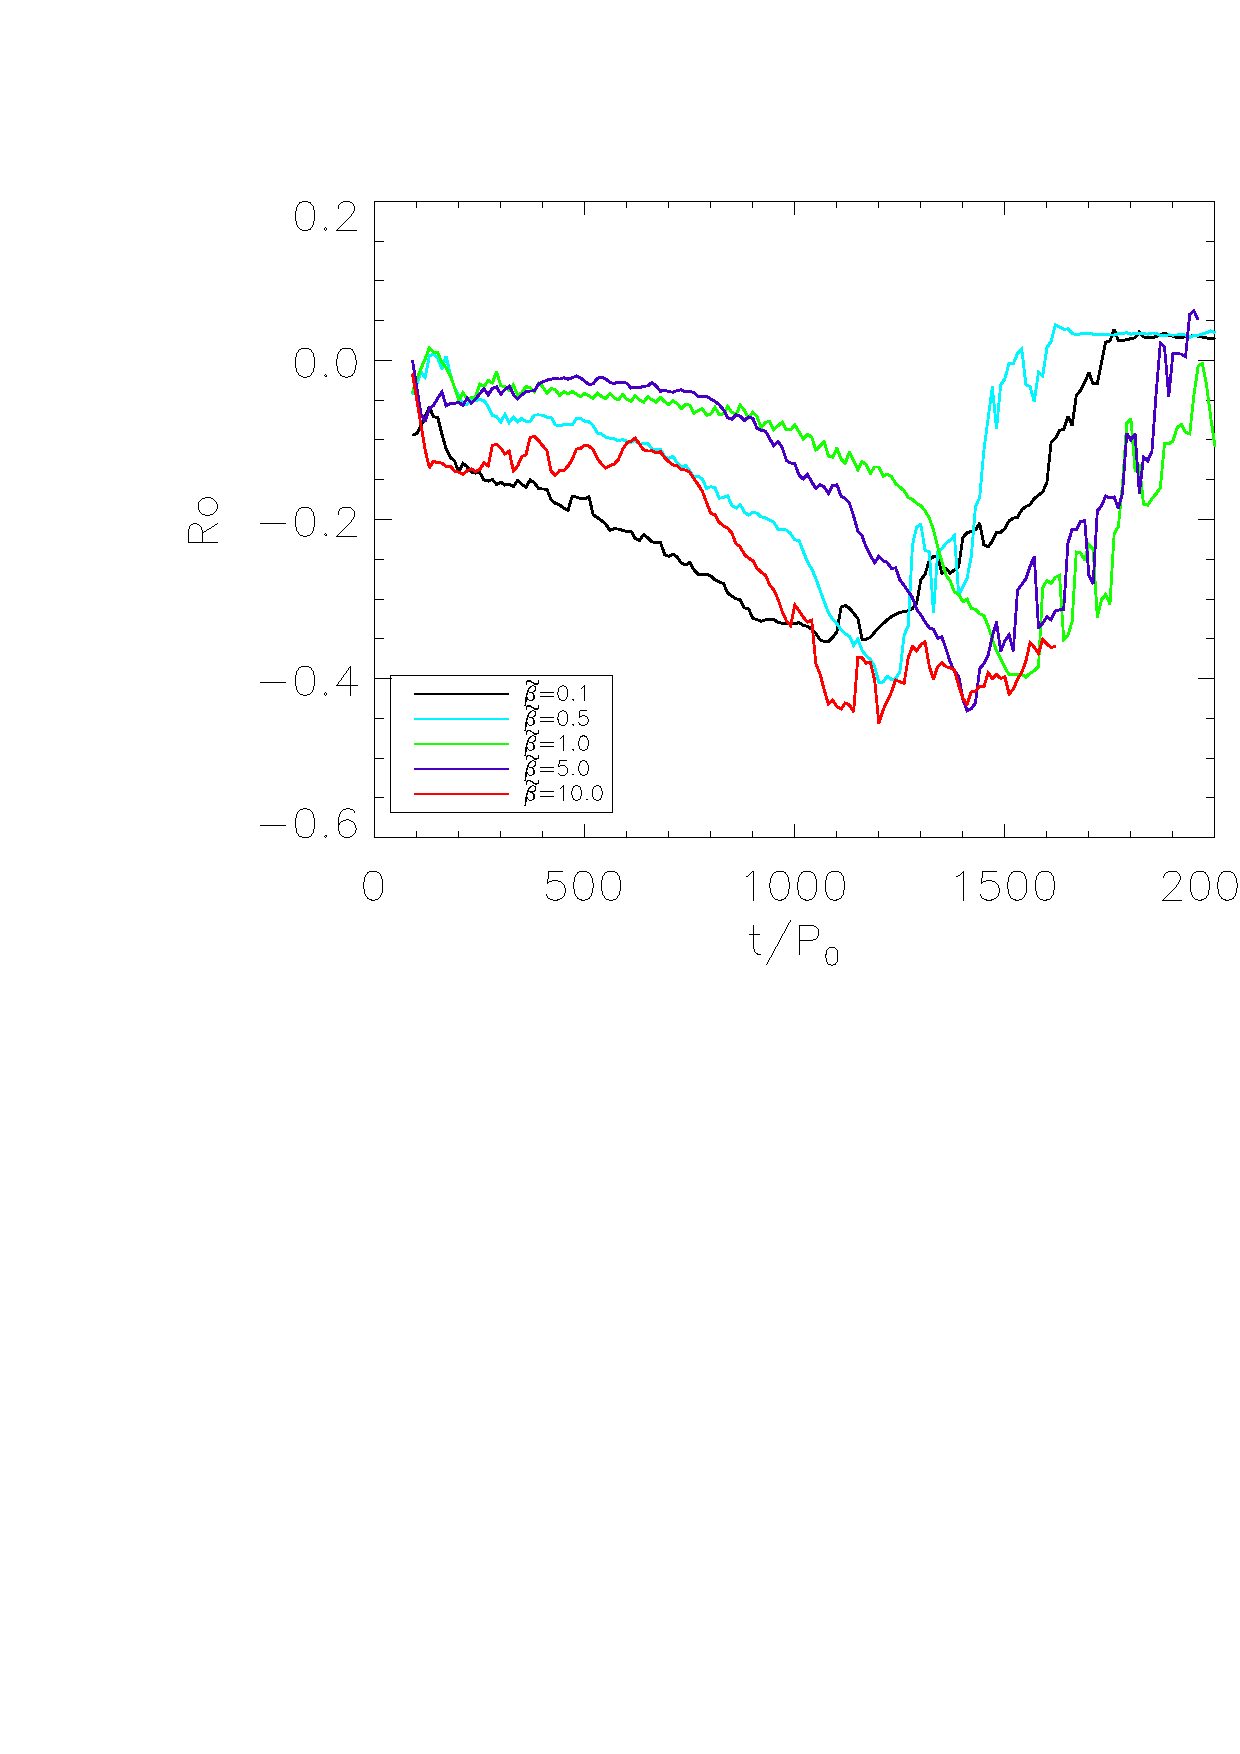
\includegraphics[width=\linewidth,clip=true,trim=0.5cm
  0cm 0cm 1cm]{figures/rossby}
  \caption{Evolution of Rossby numbers at the centres of the vortices
    formed in discs with different cooling rates. A negative Rossby
    number implies anti-cyclonic motion. Boxcar averaging
    was used to remove contributions from the planet-induced spiral shock.\label{rossbyplot}}    
\end{figure}

We find the vortices become significantly 
over-dense. Fig. \ref{overdensity} plots the surface density perturbation measured at the
vortex centres, showing $\Delta\Sigma/\Sigma_0 \gtrsim 7$ for all
cases of $\tilde\beta$ in quasi-steady state, and 
$\mathrm{max}(\Delta\Sigma/\Sigma_0)\sim 11$ for $\tilde\beta=5$.  
The maximum over-density typically increases with longer cooling
times, despite the vortices are initially weaker at formation with
increasing $\tilde{\beta}$. The large increase in the surface density
is due to vortex growth as there is continuous generation of vorticity by
planet-disc interaction. This is supported by the observation that in
the previous simulations without the planet, the amplitude of
the post-merger vortex does not grow (Fig. 
\ref{planetofflifetimeplot}).  

% We remark that the increase in the
% vortex surface density directly due to the pile-up of material at the
% gap edge (because of gap-opening) is small: the average surface density
% perturbation at vortex radial region, $r\sim r_{p}+5r_h$, is 
% $\langle\Delta\Sigma/\Sigma_0\rangle_\phi<1$.  

\begin{figure}
  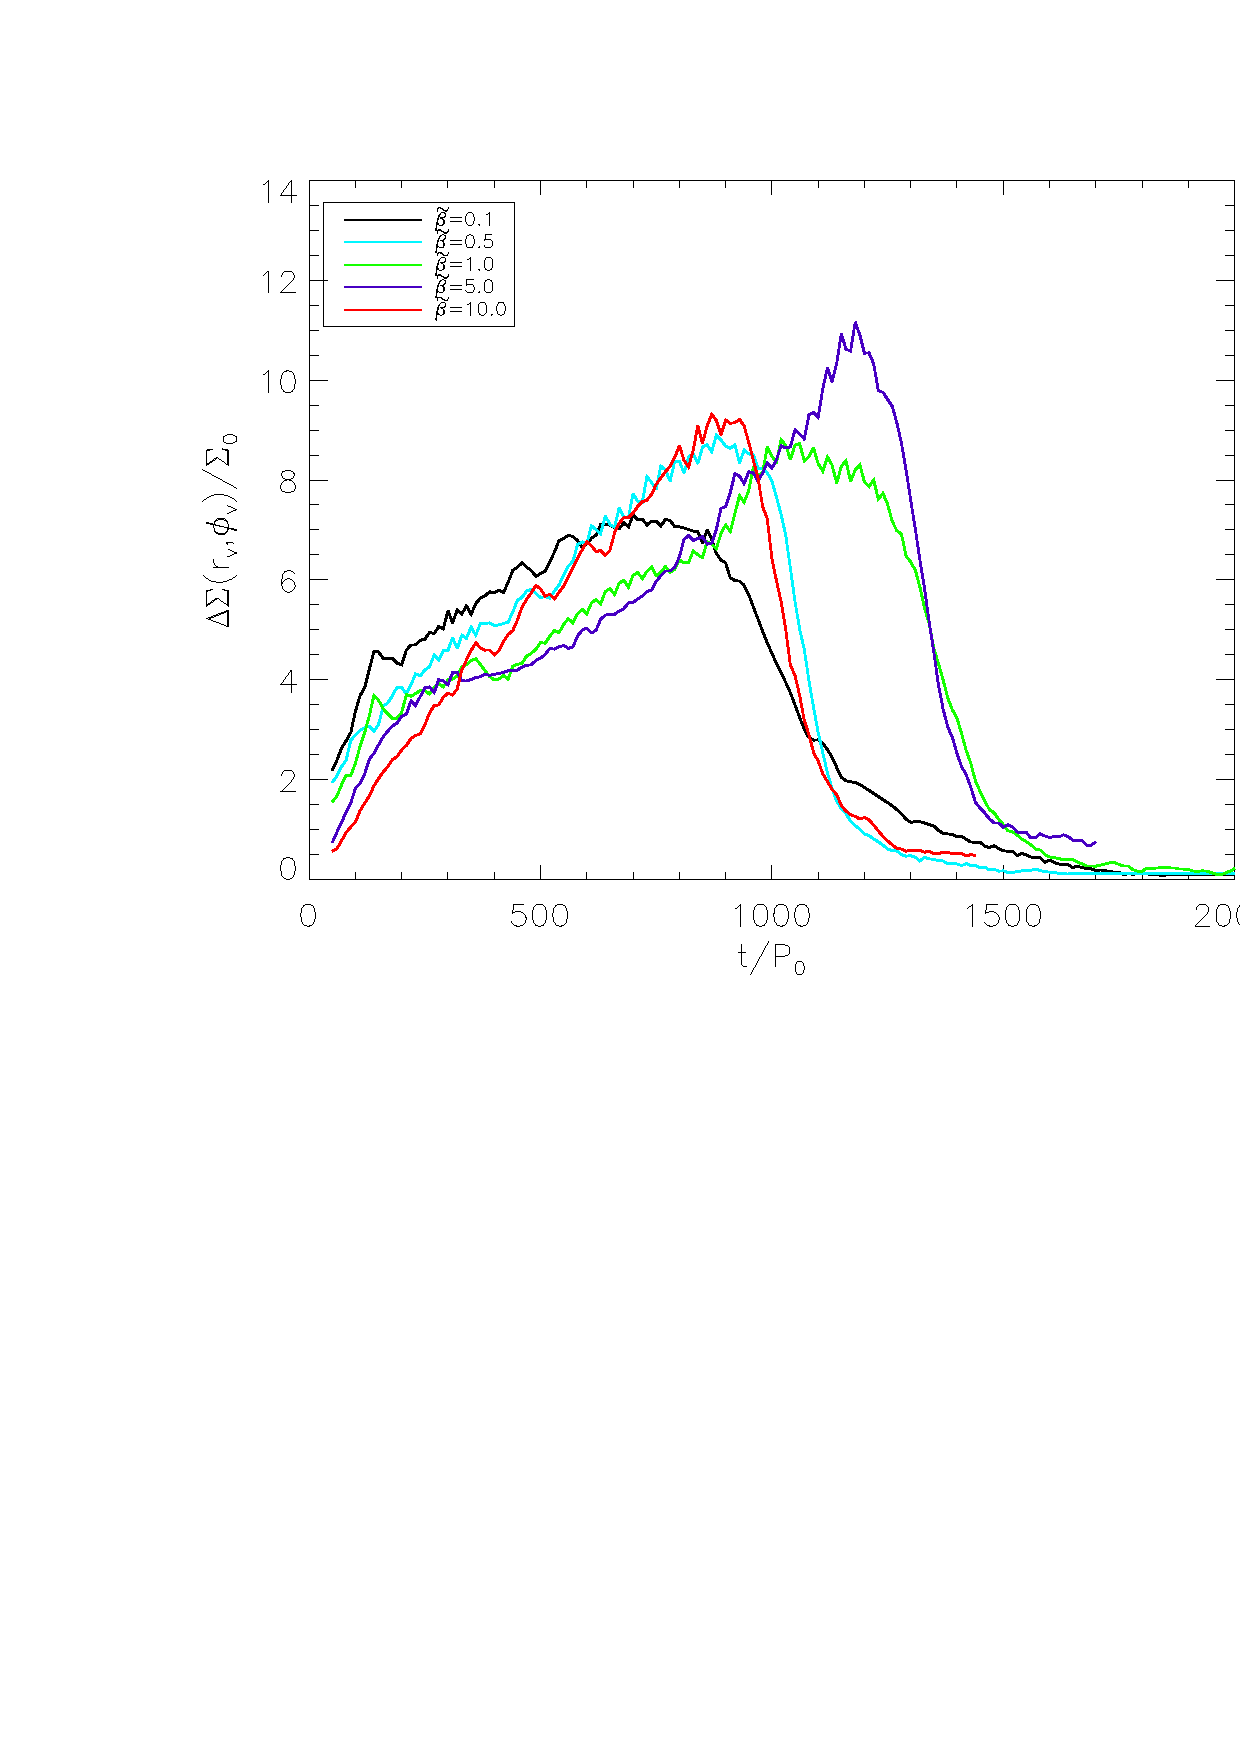
\includegraphics[width=\linewidth,clip=true,trim=0.5cm
  0cm 0cm 1cm]{figures/vortex_density}
  \caption{Average value of the relative surface density perturbation
    at vortex centres for various cooling
    times. Intial vortex overdensities decrease with cooling rate while
    vortex growth rates increase with cooling rate.
    \label{overdensity}}     
\end{figure}

Fig. \ref{lifetimeplot} shows that the duration of the quasi-steady state
varies with the cooling rate: for 
$\tilde{\beta}=0.1$ and $10$, the vortex amplitude begins to decay around
$t\sim800P_0$, while for $\tilde{\beta}=1,\,5$ the decay begins at 
$t\sim1200P_0$. This non-monotonic dependence suggests that there
exists an optimal cooling rate to maximise the vortex lifetime. We
will discuss this issue further in 
\S\ref{lifetime_discuss}. Notice the decay timescale decreases with
increasing cooling time: for $\tilde{\beta}=0.1$ it takes $\sim400P_0$
whereas for $\tilde{\beta}=10$ it takes $\sim 100P_0$ for the $m=1$
amplitude to decay significantly after reaching maximum. 


{\bf For comparison we also ran a locally isothermal simulation to
  compare with the case with rapid cooling ($\tilde{\beta}=0.01$), but
  did not observe significant vortex decay within our simulation
  timescale in the former case. This suggests there could be
  fundamental differences between the two cases.}

% {\bf may be more appropriate to quote the azimuthally averaged
%   perturbation at the location of the vortex (5-6 Hill radii from the
%   planet?): yes, this was my original idea, mistyped as 2.5
% } 

% {\bf any trend between maximum over-density achieved and cooling?: generally increasing with beta, max at beta=5} 

% {\bf question: vortex amplitude plot suggest just after linear growth,
%   vortex amplitudes are smaller with increasing beta, but later on in
%   the quasi-steady state, this trend reverses? yes. 
% }


% {\bf Perhaps a 2D snapshot of what the gap edge looks like after
%   vortex death (like the one in the poster).: Not sure if this is figure 
% you were thinking (Fig 8)
% % defer definition of  vortex lifetime to later, when we discuss it. 
% }

% \begin{figure}
%   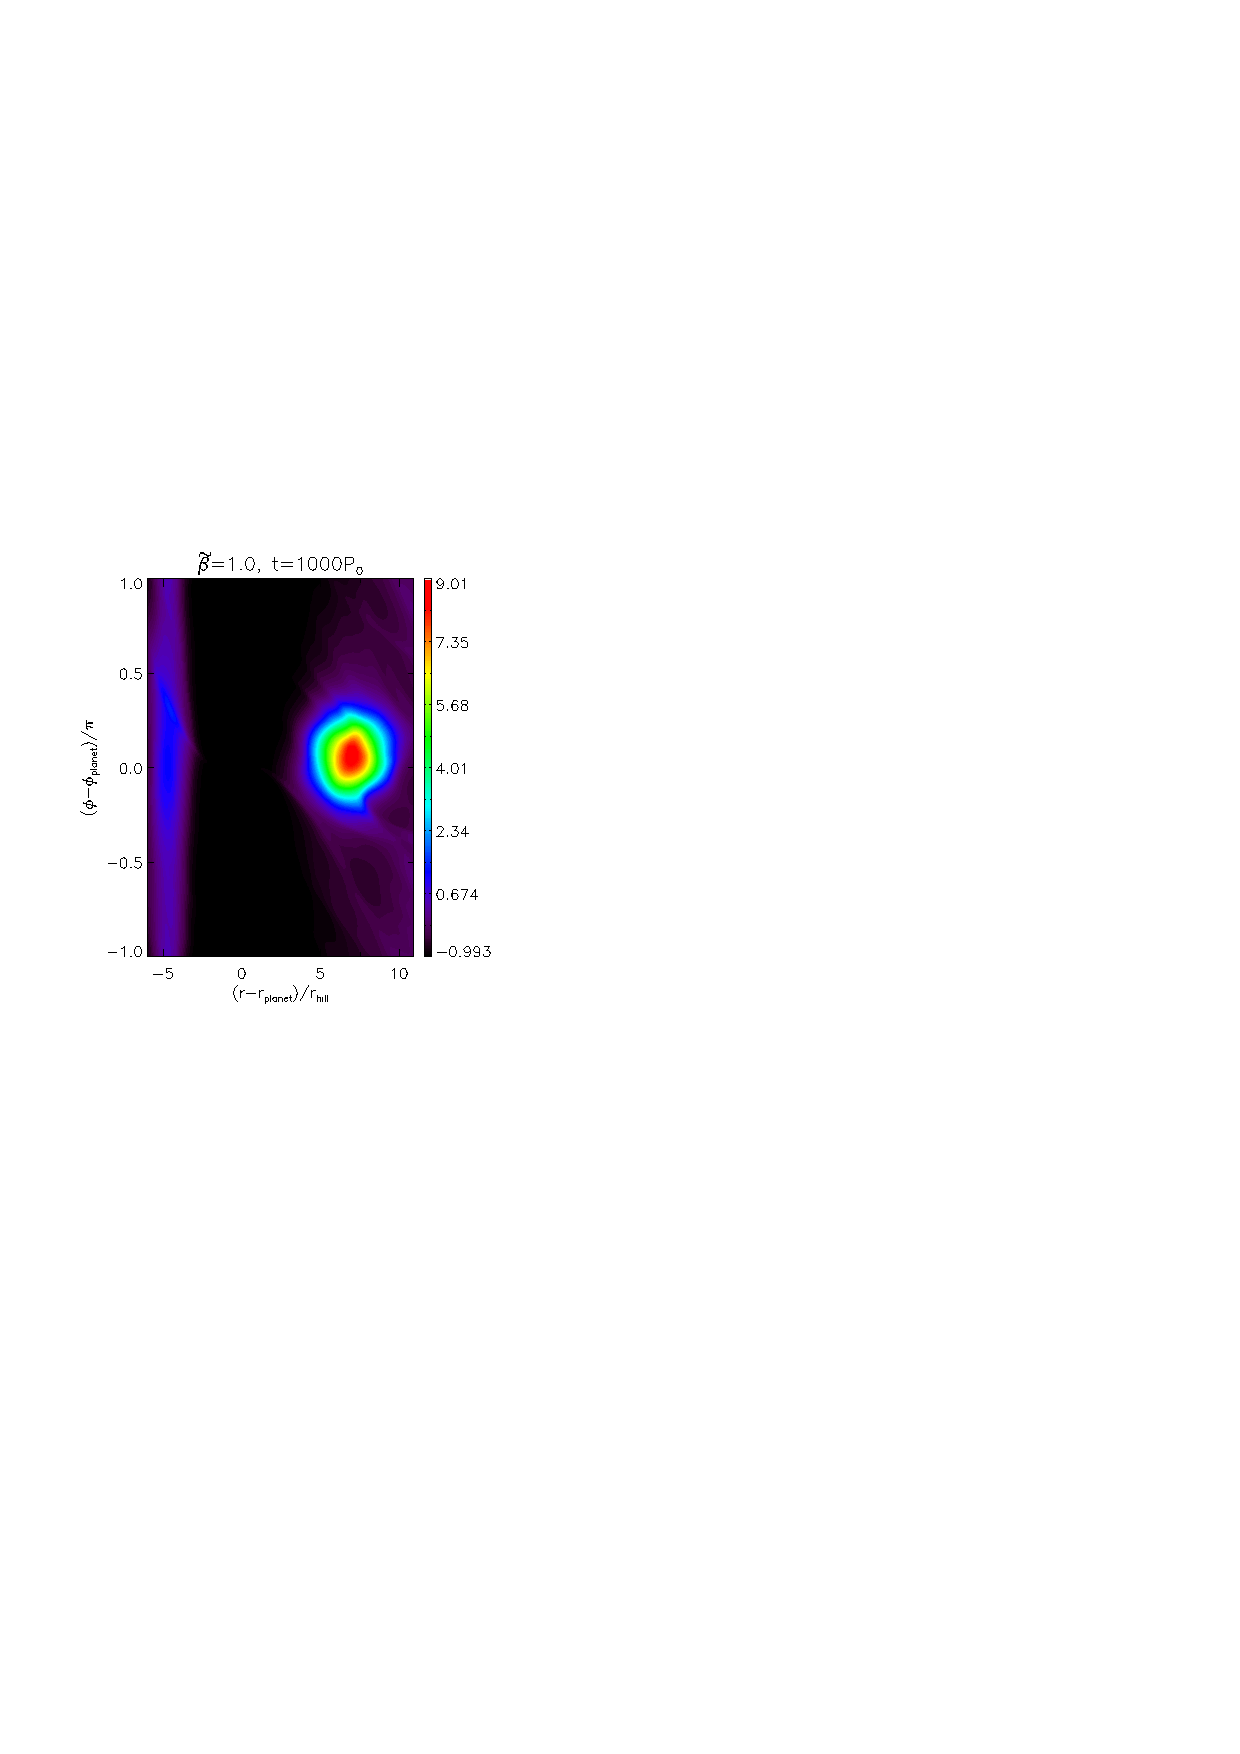
\includegraphics[width=.3\linewidth,height=.5\linewidth]{figures/analysis_sigma100}
%   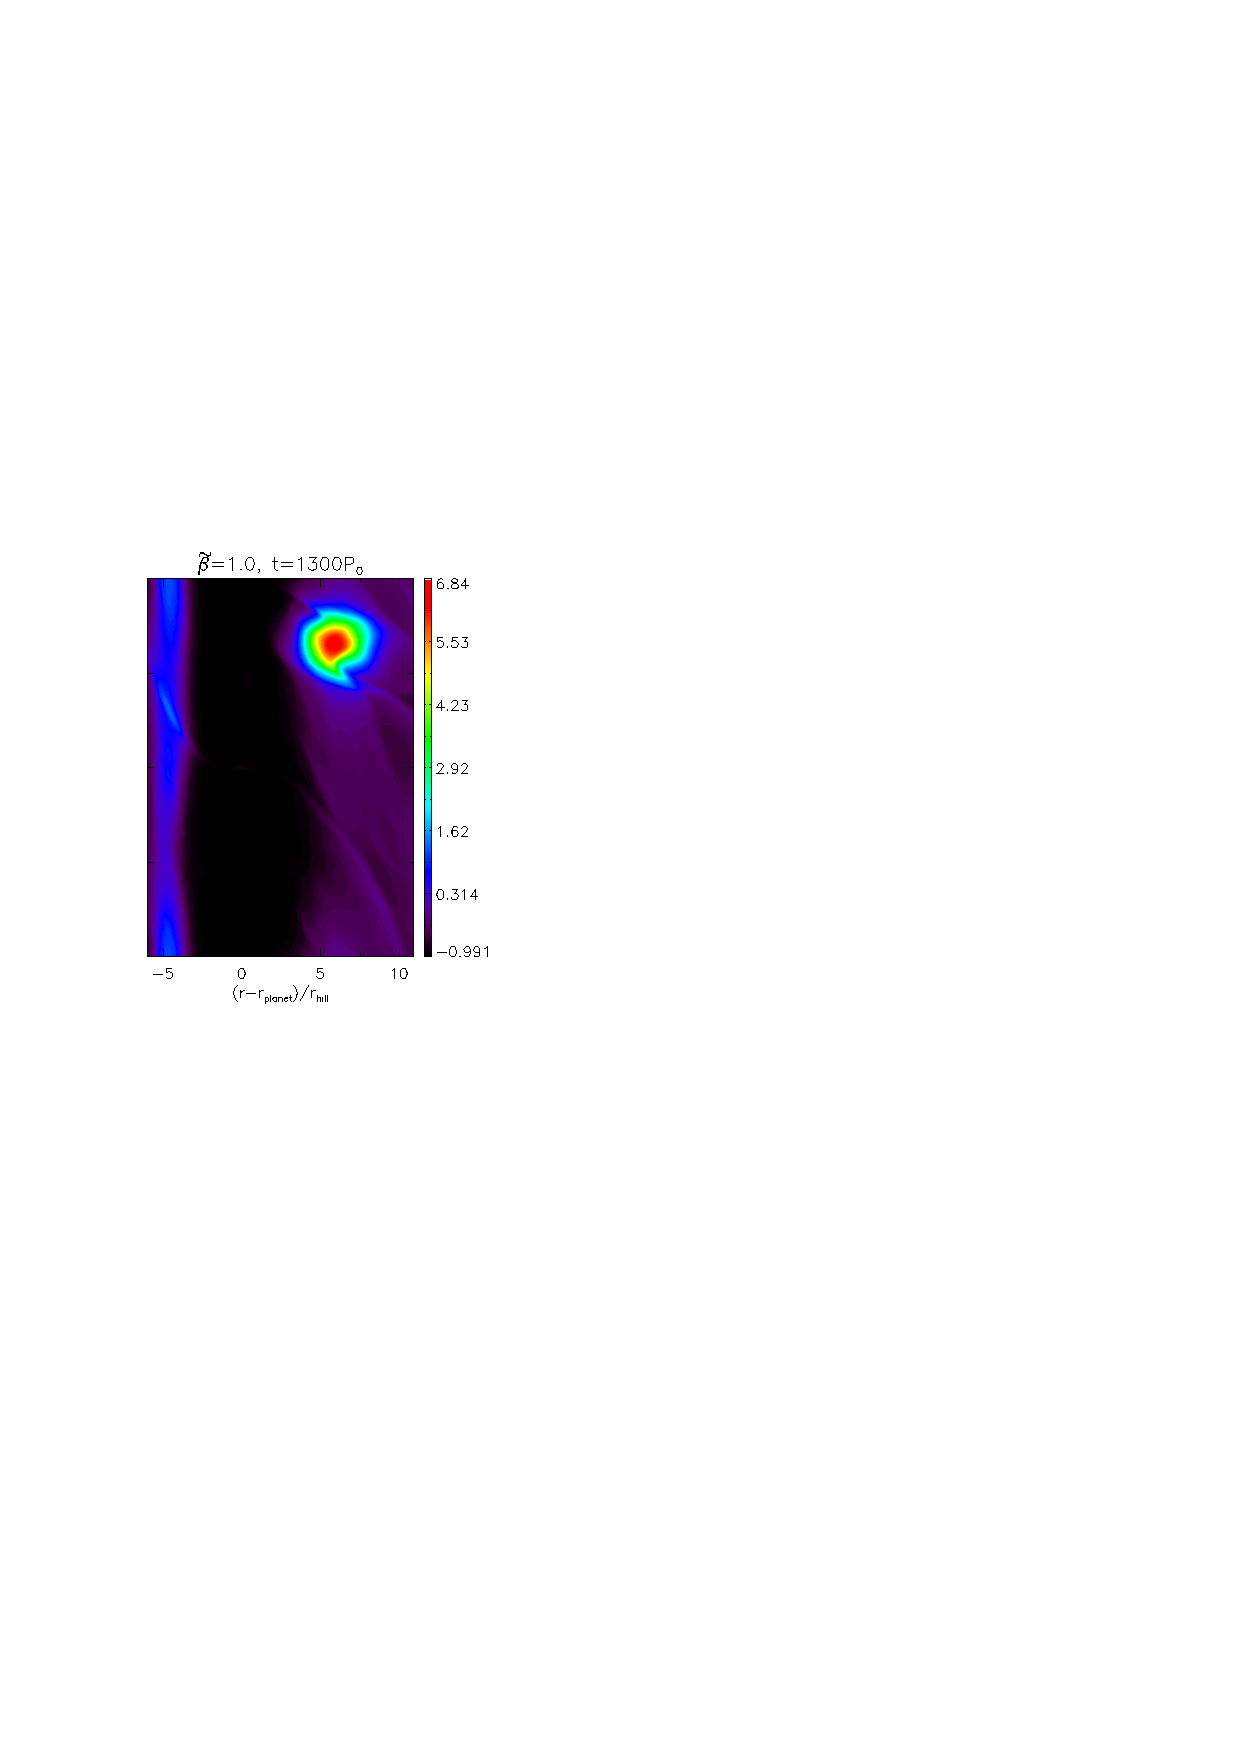
\includegraphics[width=.3\linewidth,height=.5\linewidth]{figures/analysis_sigma130}
%   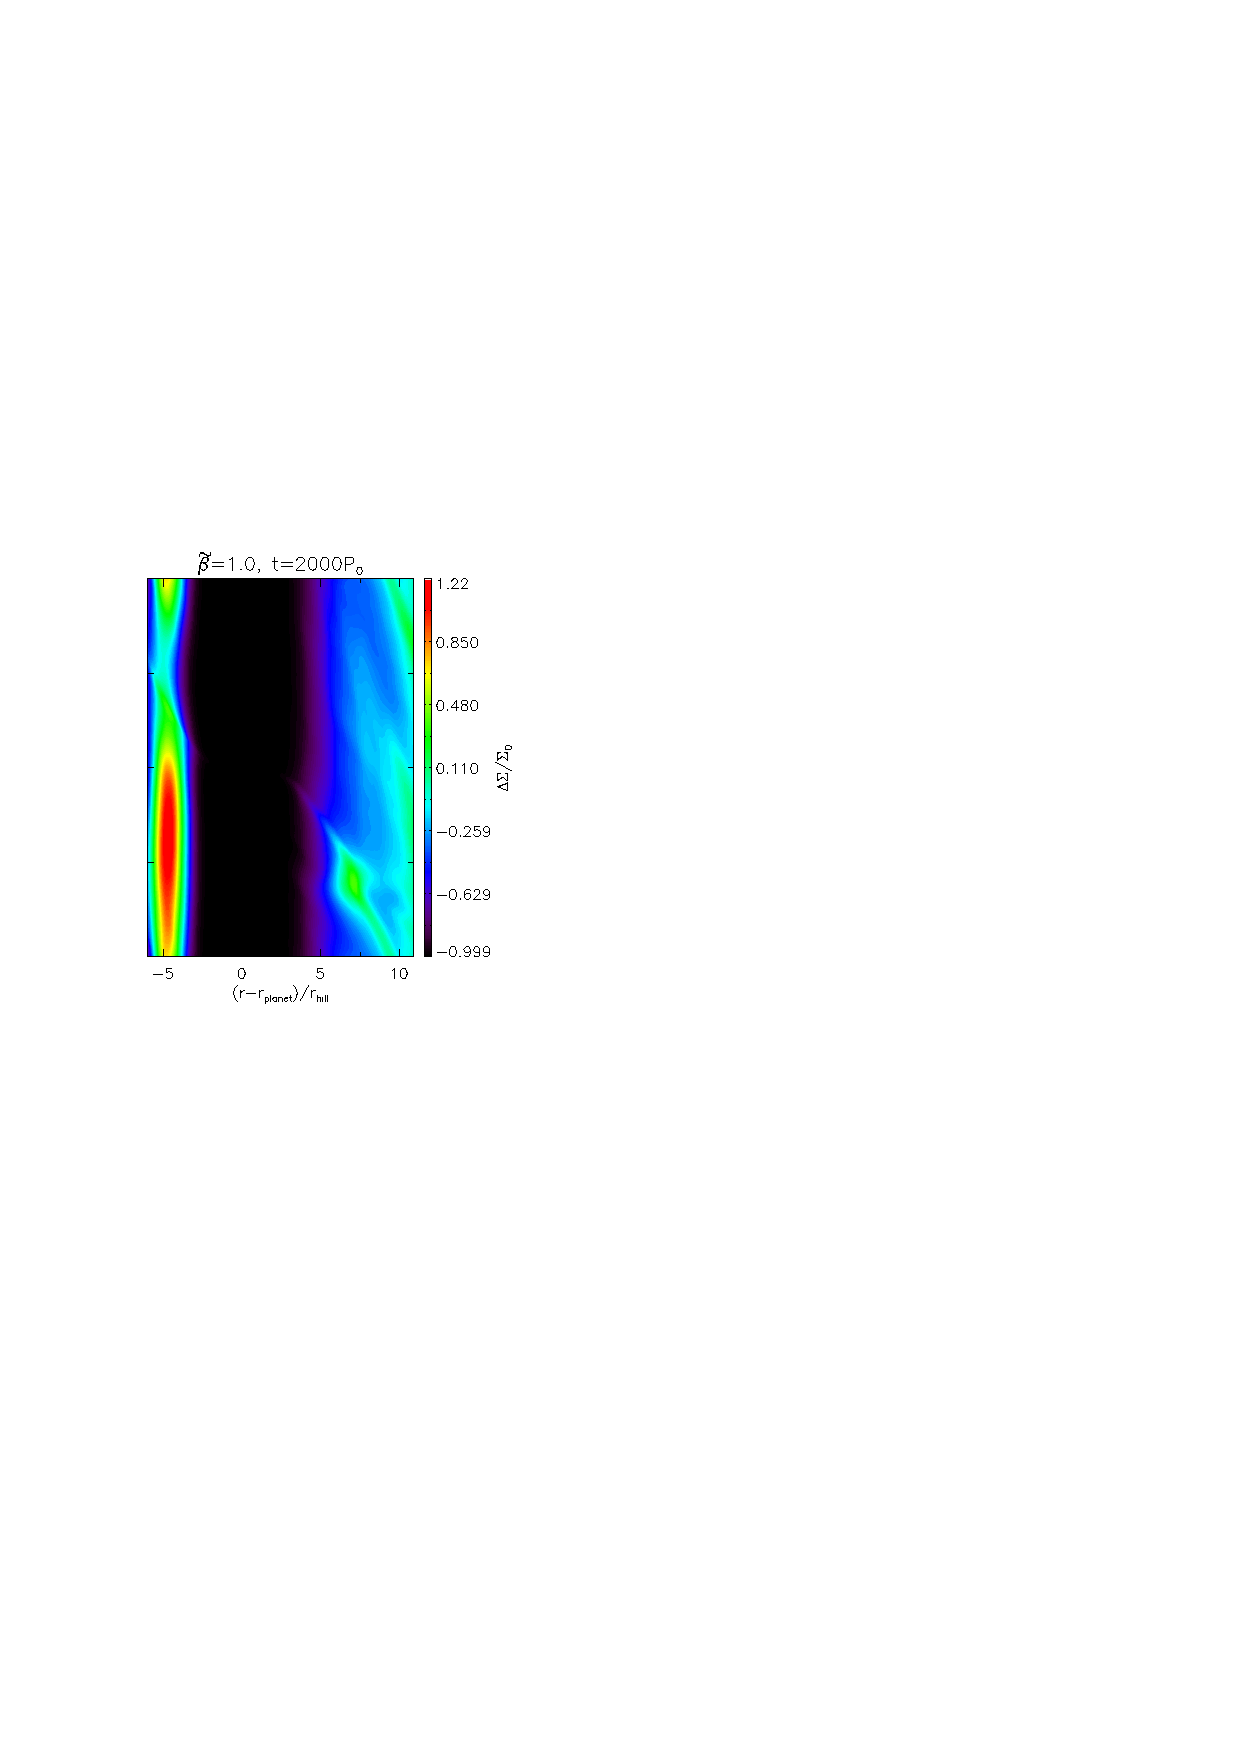
\includegraphics[width=.3\linewidth,height=.5\linewidth]{figures/analysis_sigma200}

%   \caption{2D gap profile for $\tilde\beta=1.0$ during quasisteady state (left), during dissipation (middle), and after dissipation (right).
%     \label{2dgaps}} 
% \end{figure}

\subsection{Additional analysis on vortex decay}
In this subsection we examine the vortex decay observed in our
simulations in more detail. Fig. \ref{shockplot} show snapshots
of the vortex for the case $\tilde{\beta}=1$. The plots show the surface
density perturbation and the surface density gradient during
quasi-steady state ($t=700P_0$), when the $m=1$ amplitude begins to
decrease ($t=1300P_0$) and just after the rapid amplitude decay
($t=1510P_0$). 

In quasi-steady ($t=700P_0$) the vortex is elongated with a vortex aspect ratio $ \approx 4$
, but becomes more compact approaching a ratio of 2 during its decay ($t=1310$).   
Notice in Fig. \ref{shockplot} the appearance of wakes extending from
either side of the vortex at $t=1300P_0$. These 
wakes correlate with large gradients in surface density (bottom
panel), and are first seen in the later half of the quasi-steady
state. We find the time at which 
the vortex begins to decay coincides with the emergence of these
wakes. %{\bf true statement? yes, distortion of vortex shape form wakes happens at same time}  

{\bf During the quasi-steady state the vortex 
  orbits at $r\sim r_p+6r_h$. We do not see significant
  vortex migration at this stage (true?), since the vortex is located at a
  surface density maximum, which can trap vortices
  \citep{paardekooper10}. However, simultaneous with the
  appearence of the wakes, we observe the vortex begins to migrate 
  inwards to $r\sim r_p+5r_h$. 
  % This is a result of the the spiral waves transporting
  % angular momentum to the disk (Is this true? Shocks on the inner disk
  % seem stronger so I would think it would migrate outward). 
  } 

% As the vortices grow in intensity wakes are seen to extend from them. 
During quasi-steady state the average value of the surface density gradient
along the wakes is $|w_s\nabla\Sigma/\Sigma| \sim 0.4 $, where 
$w_s\simeq0.1$ (code units) is a typical length scale of 
the surface density variation across the wake.   
Just before the $m=1$ amplitude begins to decrease, we observe this quantity
sharply increases to $ \sim 0.6 $, and remains around this value
until the vortex dies out, at which point the associated Rossby number
begins decreasing to zero. {\bf After the 
  vortex reaches small amplitudes ($1\lesssim\Delta\Sigma/\Sigma$), it 
  migrates out to $r\sim r_p+ 6.5 r_h$. 
}
%{\bf :check}.   

% {\bf rough estimate of
%   vortex aspect-ratio in the three snapshots? 
%   (length/width, by inspection is ok):trend of decreasing aspect ratio is common for all beta}  
% {\bf this quantity has dimensions of 1/length, preferable to quote something
%   dimensionless, or say `in code units': used shock width since relavant
%  distance, since small may appear to weaken value/argument}

\begin{figure}
  \subfigure{
    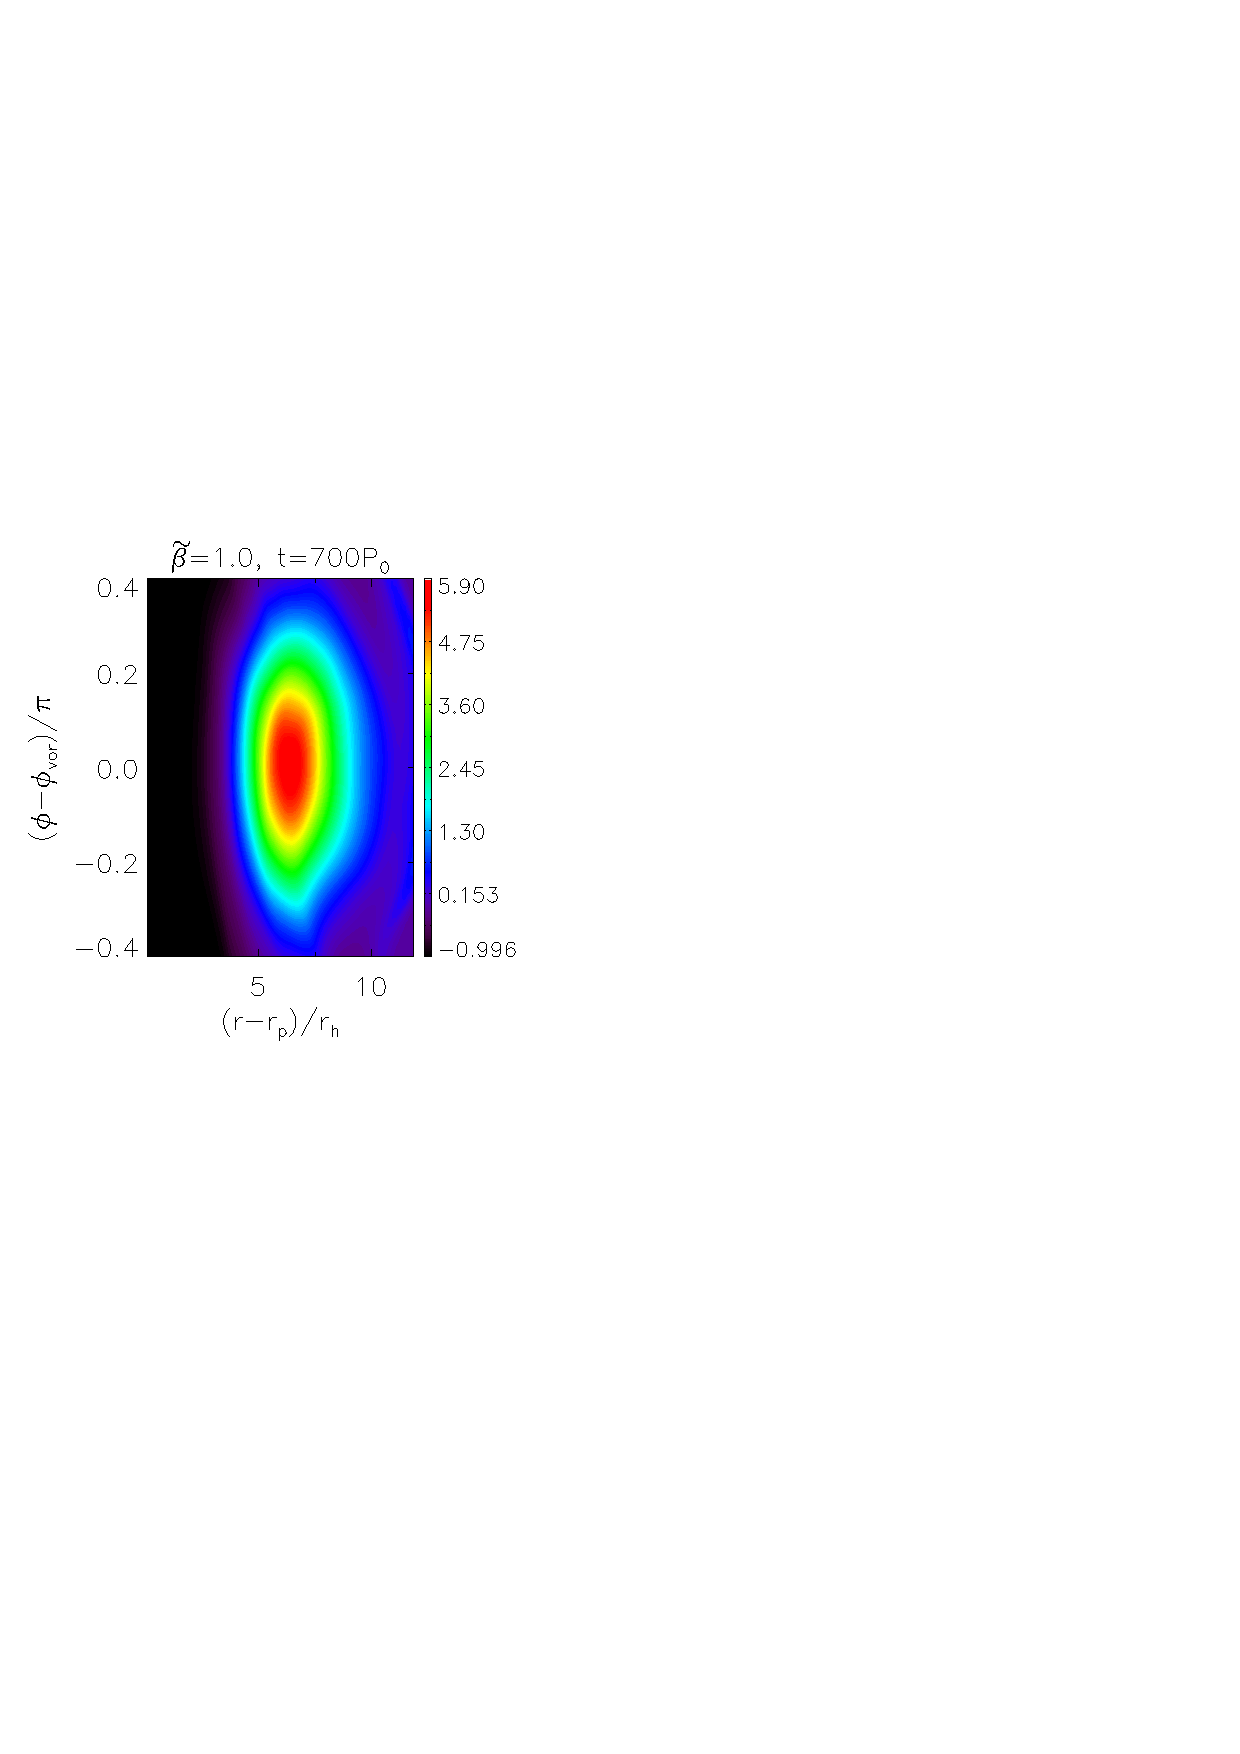
\includegraphics[width=0.3\linewidth]{figures/shock1}
  }
  \hfill
  \subfigure{
    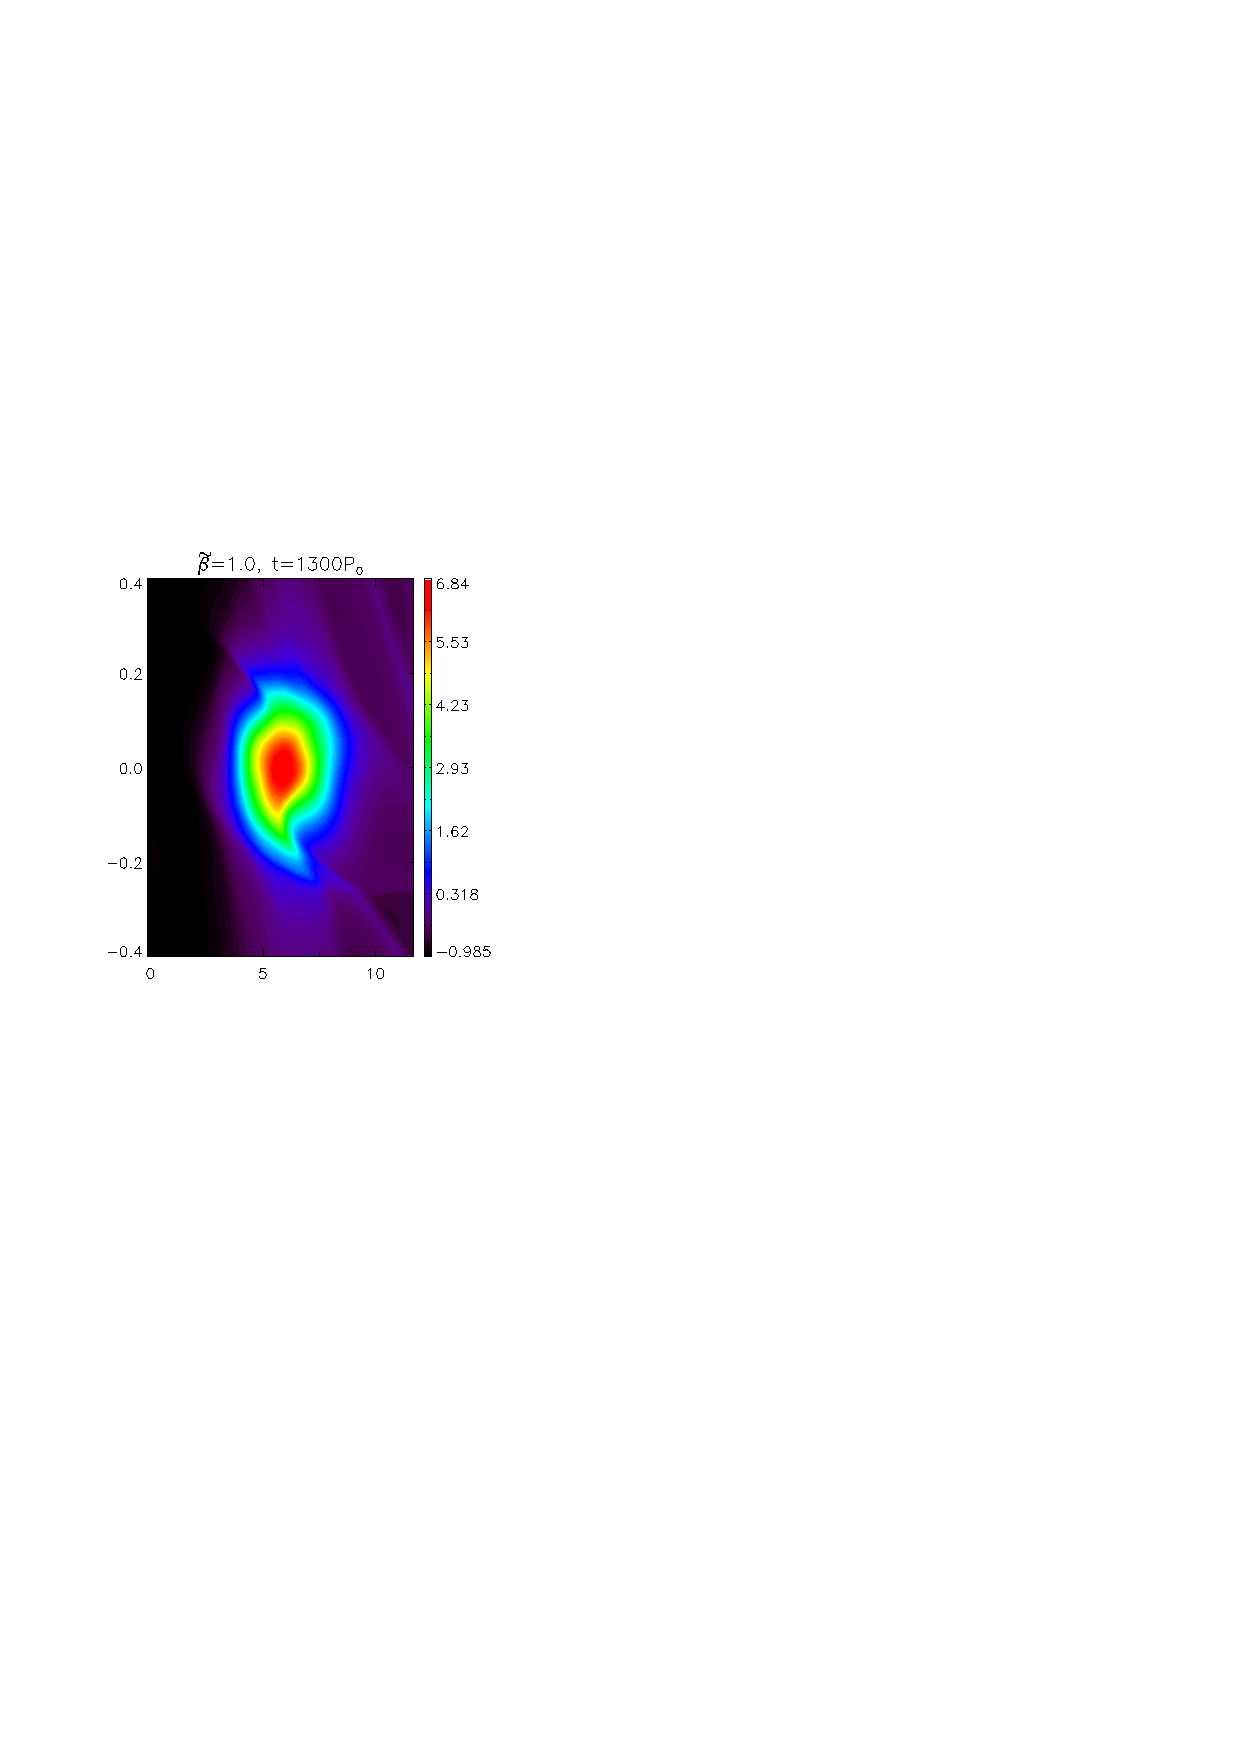
\includegraphics[width=0.3\linewidth]{figures/shock2}
  }
  \hfill
  \subfigure{
    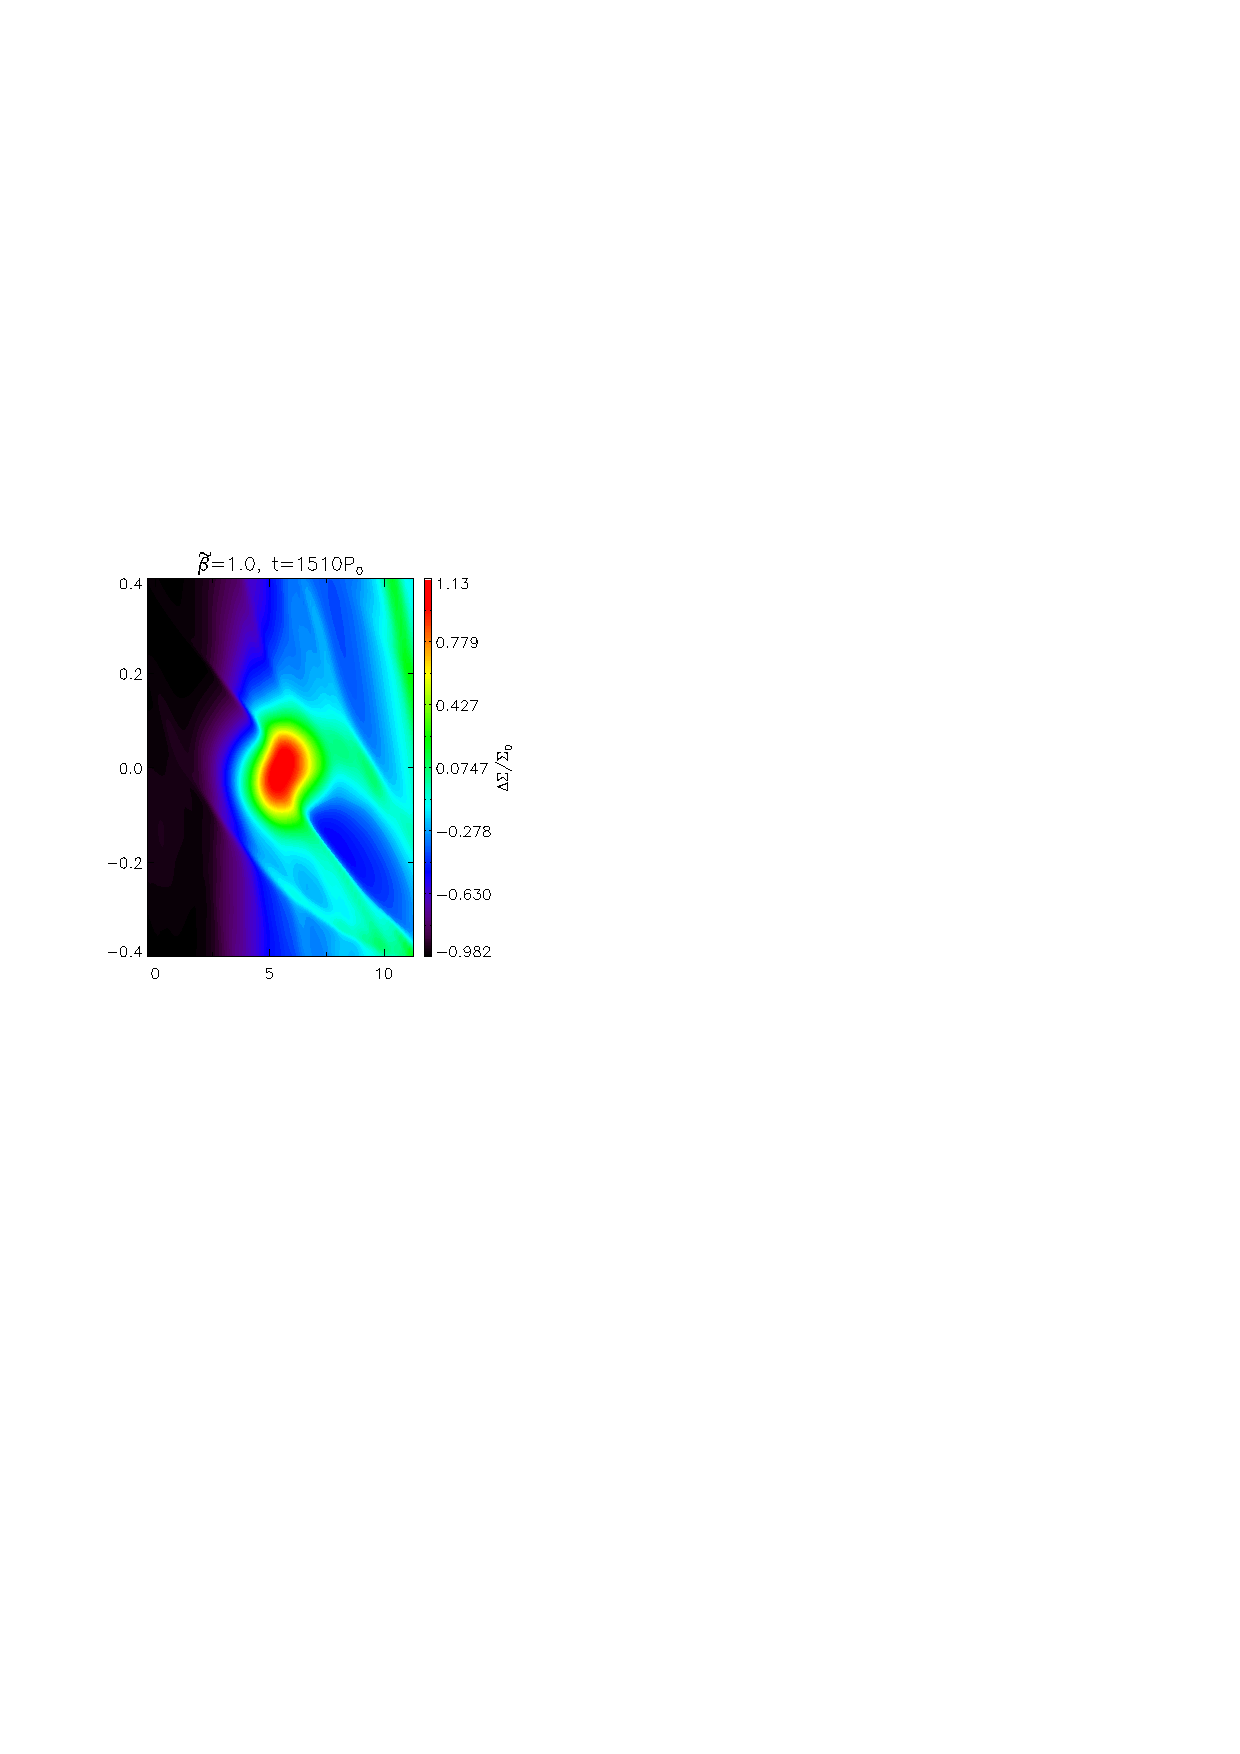
\includegraphics[width=0.3\linewidth]{figures/shock3}
  } \\[-0.98cm]
  \subfigure{
    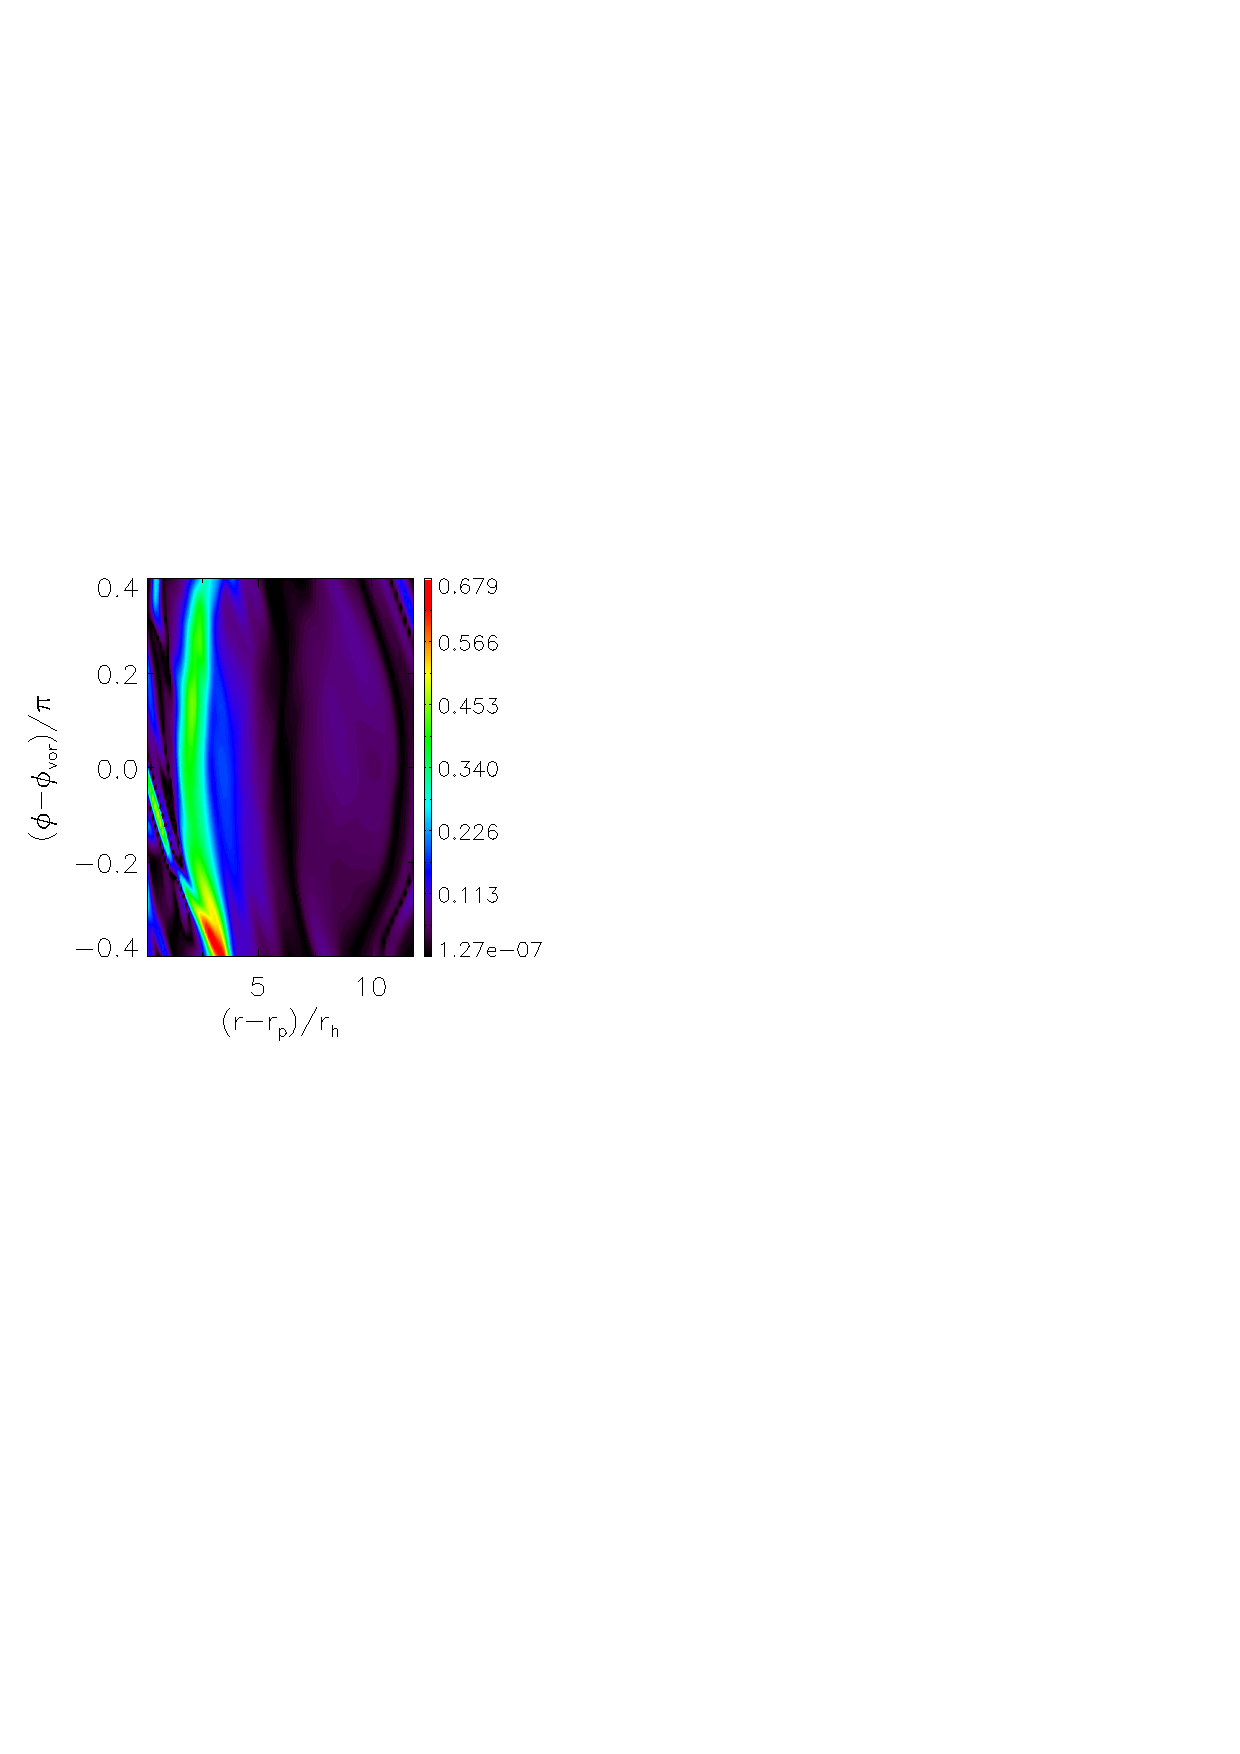
\includegraphics[width=0.3\linewidth]{figures/shock4}
  }
  \hfill
  \subfigure{
    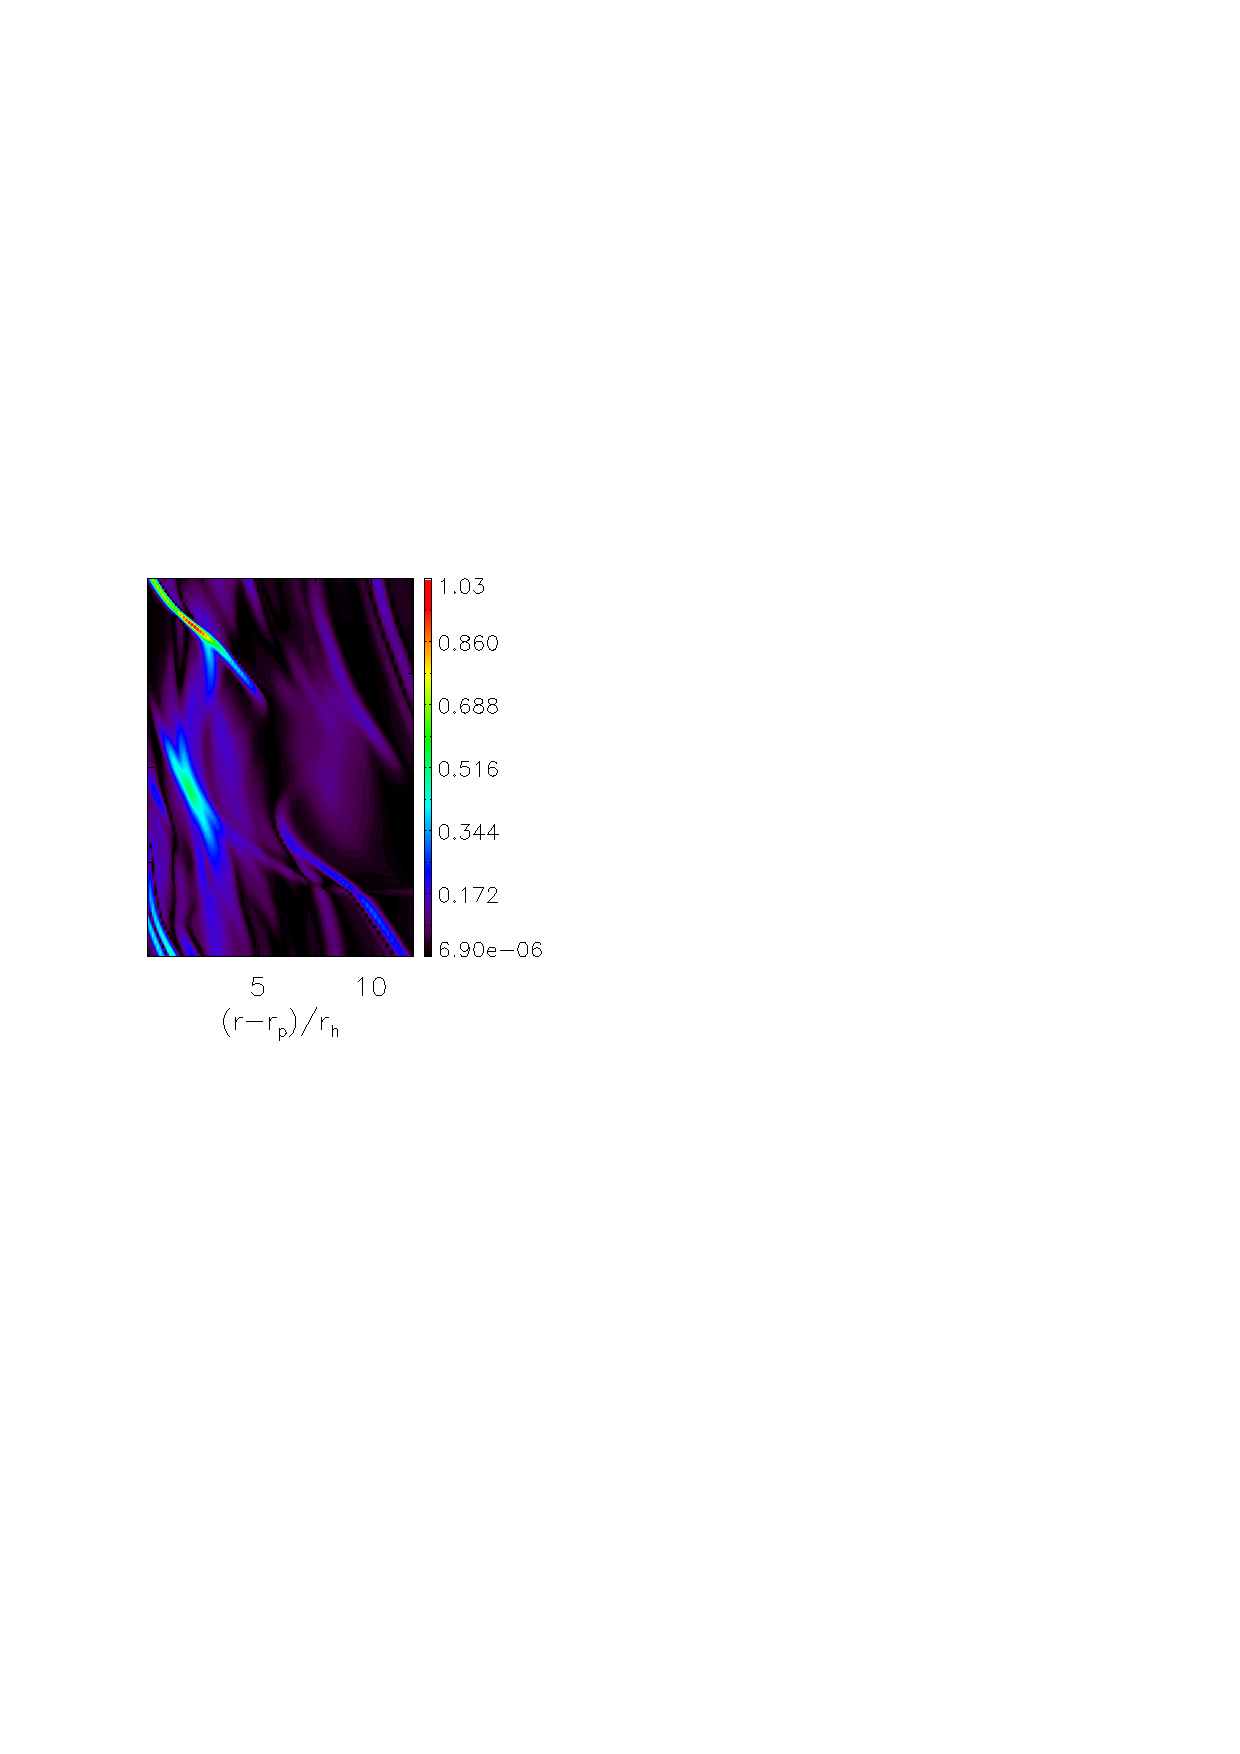
\includegraphics[width=0.3\linewidth]{figures/shock5}
  }
  \hfill
  \subfigure{
    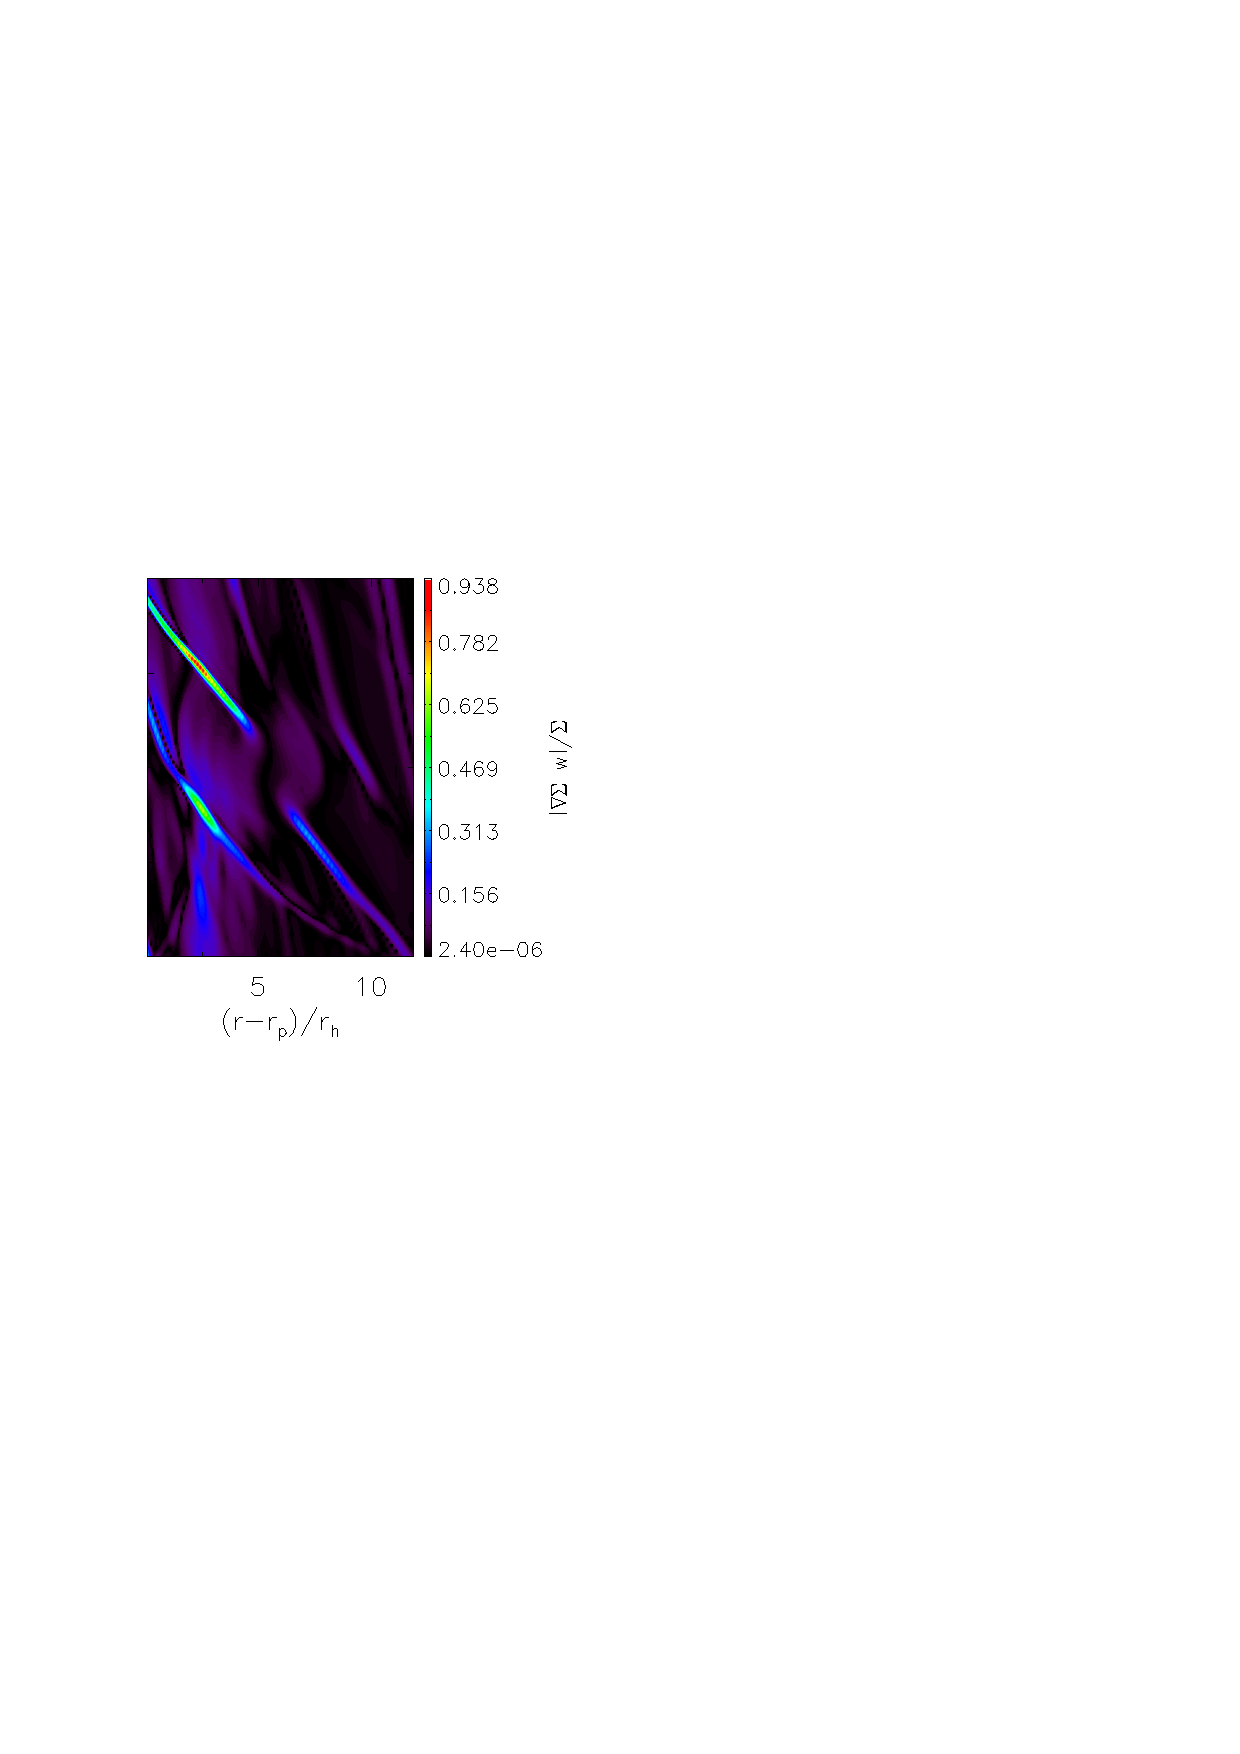
\includegraphics[width=0.3\linewidth]{figures/shock6}
  } 
  \caption{The vortex in the case with $\tilde{\beta}=1$
    during quasi-steady state (left), start of decay 
    (middle), and just after the decay in the $m=1$ amplitude
    (right). The surface density perturbation
    (top) and the associated surface density gradient (bottom) are
    shown. Wake like features corresponding to large density gradients
    are found to originate from the vortices during the late phase of 
    their quasi-steady states and into dissipation times.
    This plot is to be considered in conjunction with
    Fig. \ref{lifetimeplot}. 
    \label{shockplot}}
  % Large surface density gradients become prominant
  % around vortex during dissipation} 
\end{figure}

We also measured large increases in the Mach number near
the vortex as the $m=1$ surface density amplitude reaches maximum and begins to decay. 
Fig. \ref{machplot} plots the Mach number $M=|\bm{v} -
\bm{v}_\mathrm{vor}|/c_s$, where 
$\bm{v}_\mathrm{vor}$ corresponds to the bulk velocity of the vortex
around the disc. Values in Fig. \ref{machplot} have been averaged over
a region within $2H$ of the vortex centre. 
During the quasi-steady state the Mach number increases 
steadily, and for all cases $M$ maximises about
% with larger growth rate for higher $\tilde\beta$.
$\sim 100P_0$ after the start the $m=1$ surface density
amplitude starts to decay. 
% {\bf check if  statement is true}

Putting the above observations together, we suggest that vortex decay
(in the $m=1$ surface density amplitude) is due to shock formation by
the vortex. When the vortex reaches large amplitude, it begins
to induce shocks in the surrounding fluid, as supported by the
increase in Mach number and the appearance of wakes with large surface
density gradients. The vortex may lose energy through shock
dissipation. In addition, a strong vortex (or shock formation) 
can smooth out the gap structure that originally gave rise to the
RWI, which would oppose vortex growth. We examine this below.

\begin{figure}
  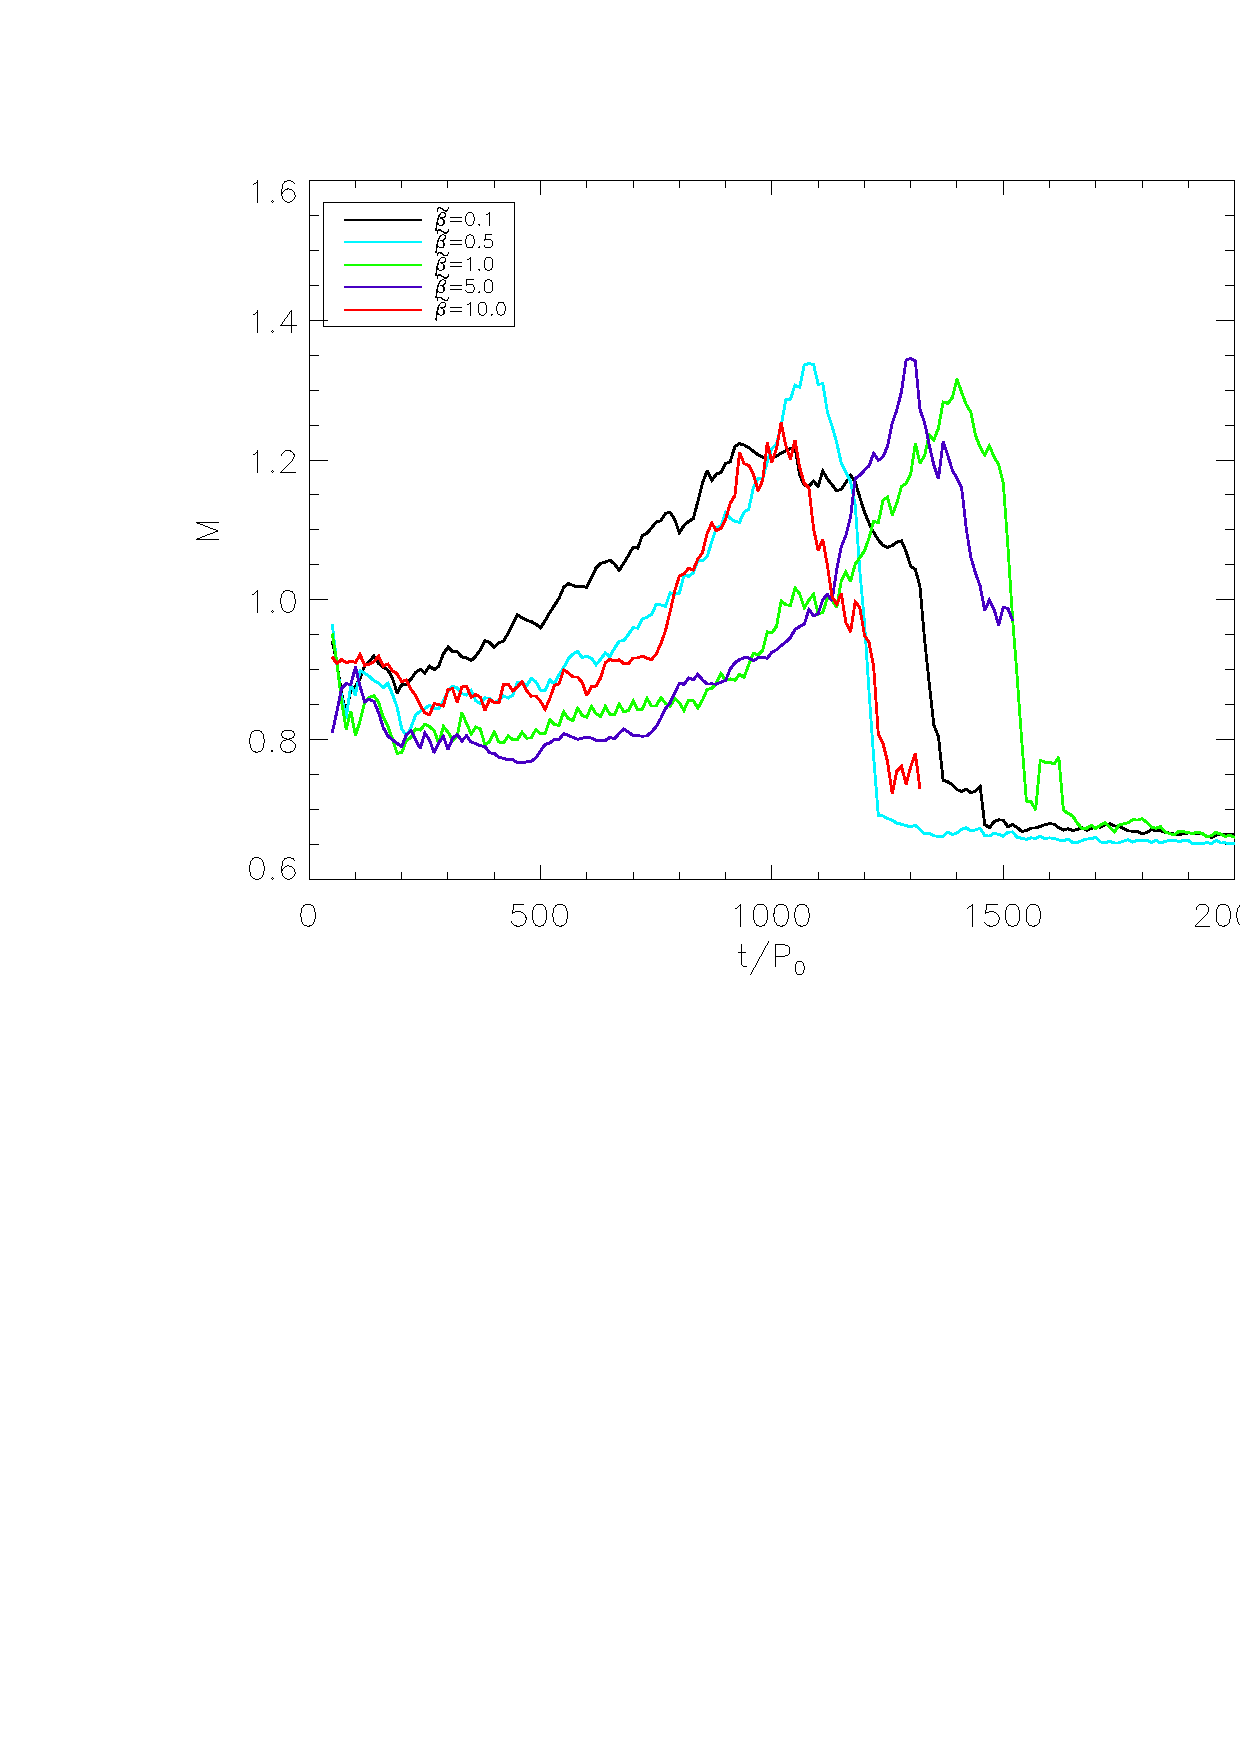
\includegraphics[width=\linewidth]{figures/mach}
  \caption{Mach number relative to
    the vortex, averaged over a region within $2H$ of the  
    vortex centre with respect to time. This plot can be compared to the evolution of the
    vortex amplitude shown in Fig. \ref{lifetimeplot}.
    \label{machplot}}
\end{figure}

\subsection{Vortex decay and gap structure}  
We find vortex decay modifies the gap
structure. Fig. \ref{gap_smoothed} shows the gap profile before and
after vortex decay for the case $\tilde{\beta}=1$. The vortex resides
around the local surface density maximum at the outer gap edge ($r\sim r_p +
6r_h$). We see that after its amplitude has decayed ($t\sim1500P_0$,   
Fig. \ref{lifetimeplot}), this local surface density maximum is also 
smoothed out.

\begin{figure}
  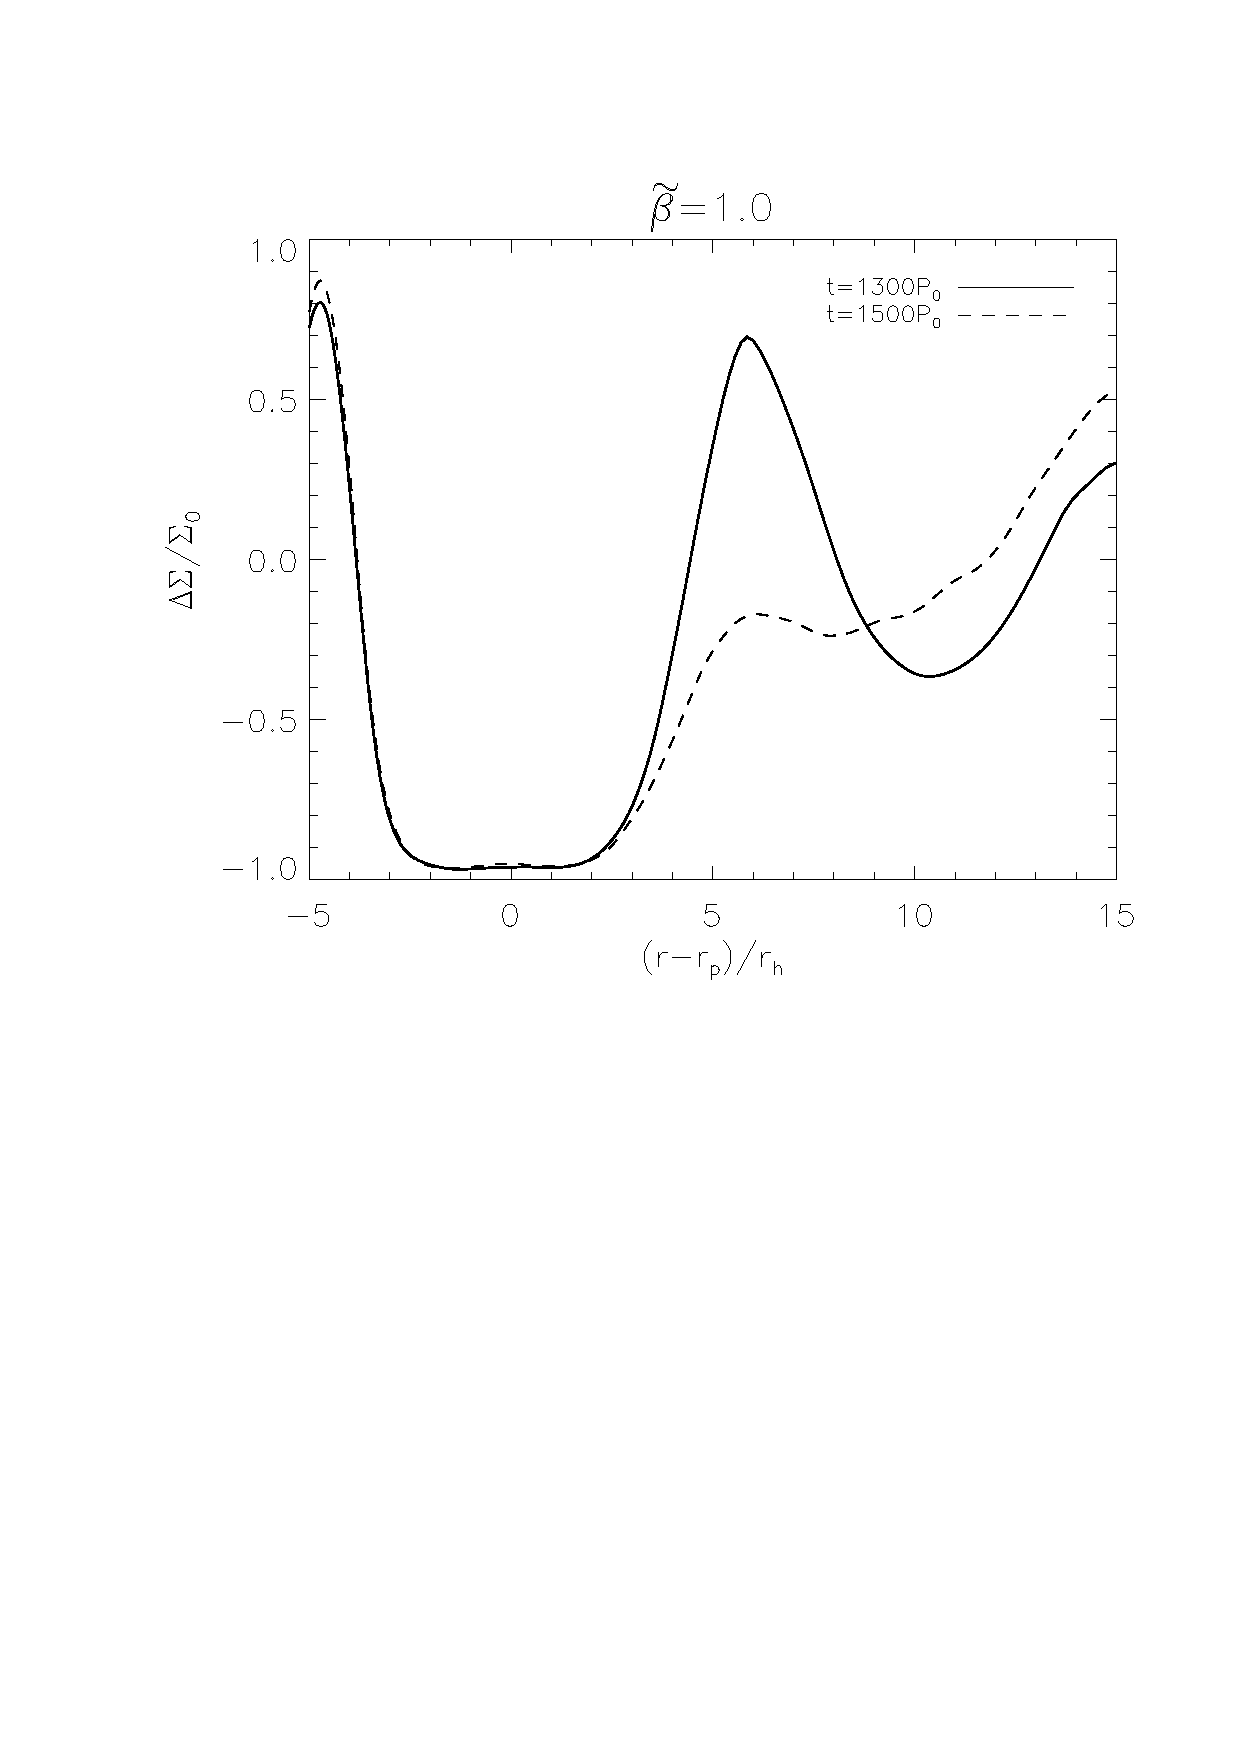
\includegraphics[width=\linewidth]{figures/gapchange}
  \caption{Azimuthally averaged profiles of the relative surface
    density perturbations for  $\tilde\beta=1.0$
    before (solid) and after vortex decay
    (dashed). Alongside drastic reduction in the outer gap maxima, vortex decay
    smoothens out the sharp outer gap edge.
    \label{gap_smoothed}} 
\end{figure}

We characterise the smoothness of the outer gap edge with a dimensionless
gap edge gradient parameter
\begin{align}
  \delta\Sigma(t)= \la \frac{\partial \langle \Sigma(t,r)
    \rangle_{\phi}}{\partial r} \cdot \frac{r}{\langle \Sigma(t=0,r)
    \rangle_{\phi}} \ra_{\Delta r}  
\end{align}
where $\Delta r = r\in [r_p,r_p + 6r_h]$ is the radial range of averaging, spanning
from centre of the gap to the radius of the surface density maximum.
A larger $\delta \Sigma$ characterises a sharper gap edge and  
larger local surface density maxima.   

A plot of the gradient parameter over time
for the $\tilde\beta=1.0$ case is shown in Fig. \ref{smoothnessplot}.
During vortex decay, the outer gap edge is 
drastically smoothed out, changing from a value of $\delta\Sigma=1.2$ during
quasi-steady state to $0.4$ after dissipation. 
%and we find that the gap edge is smoothed during this
%process. 

This can be interpreted as the vortex providing a viscosity;  
and we measure a typical alpha viscosity $\alpha = O(10^{-2})$
associated with the vortex. This acts against gap-opening
by the planet {\bf, and smooths out the outer surface density bump,    
} so the condition for the RWI 
becomes less favourable. {\bf In
  order to re-launch the RWI, the surface density bump should
  reform. However, this is difficult as there is no more material
  in the planet's vicinity to clear out (Fig. \ref{gap_smoothed}).} {\bf This may} may explain
why vortices do  not reform again (at least within the simulation timescale). 
{\bf what is aspect-ratio at outer gap edge after full decay?}

%Thus, the
%time needed for the vortex to grow to sufficient amplitude to modify
%the gap structure  

\begin{figure}
  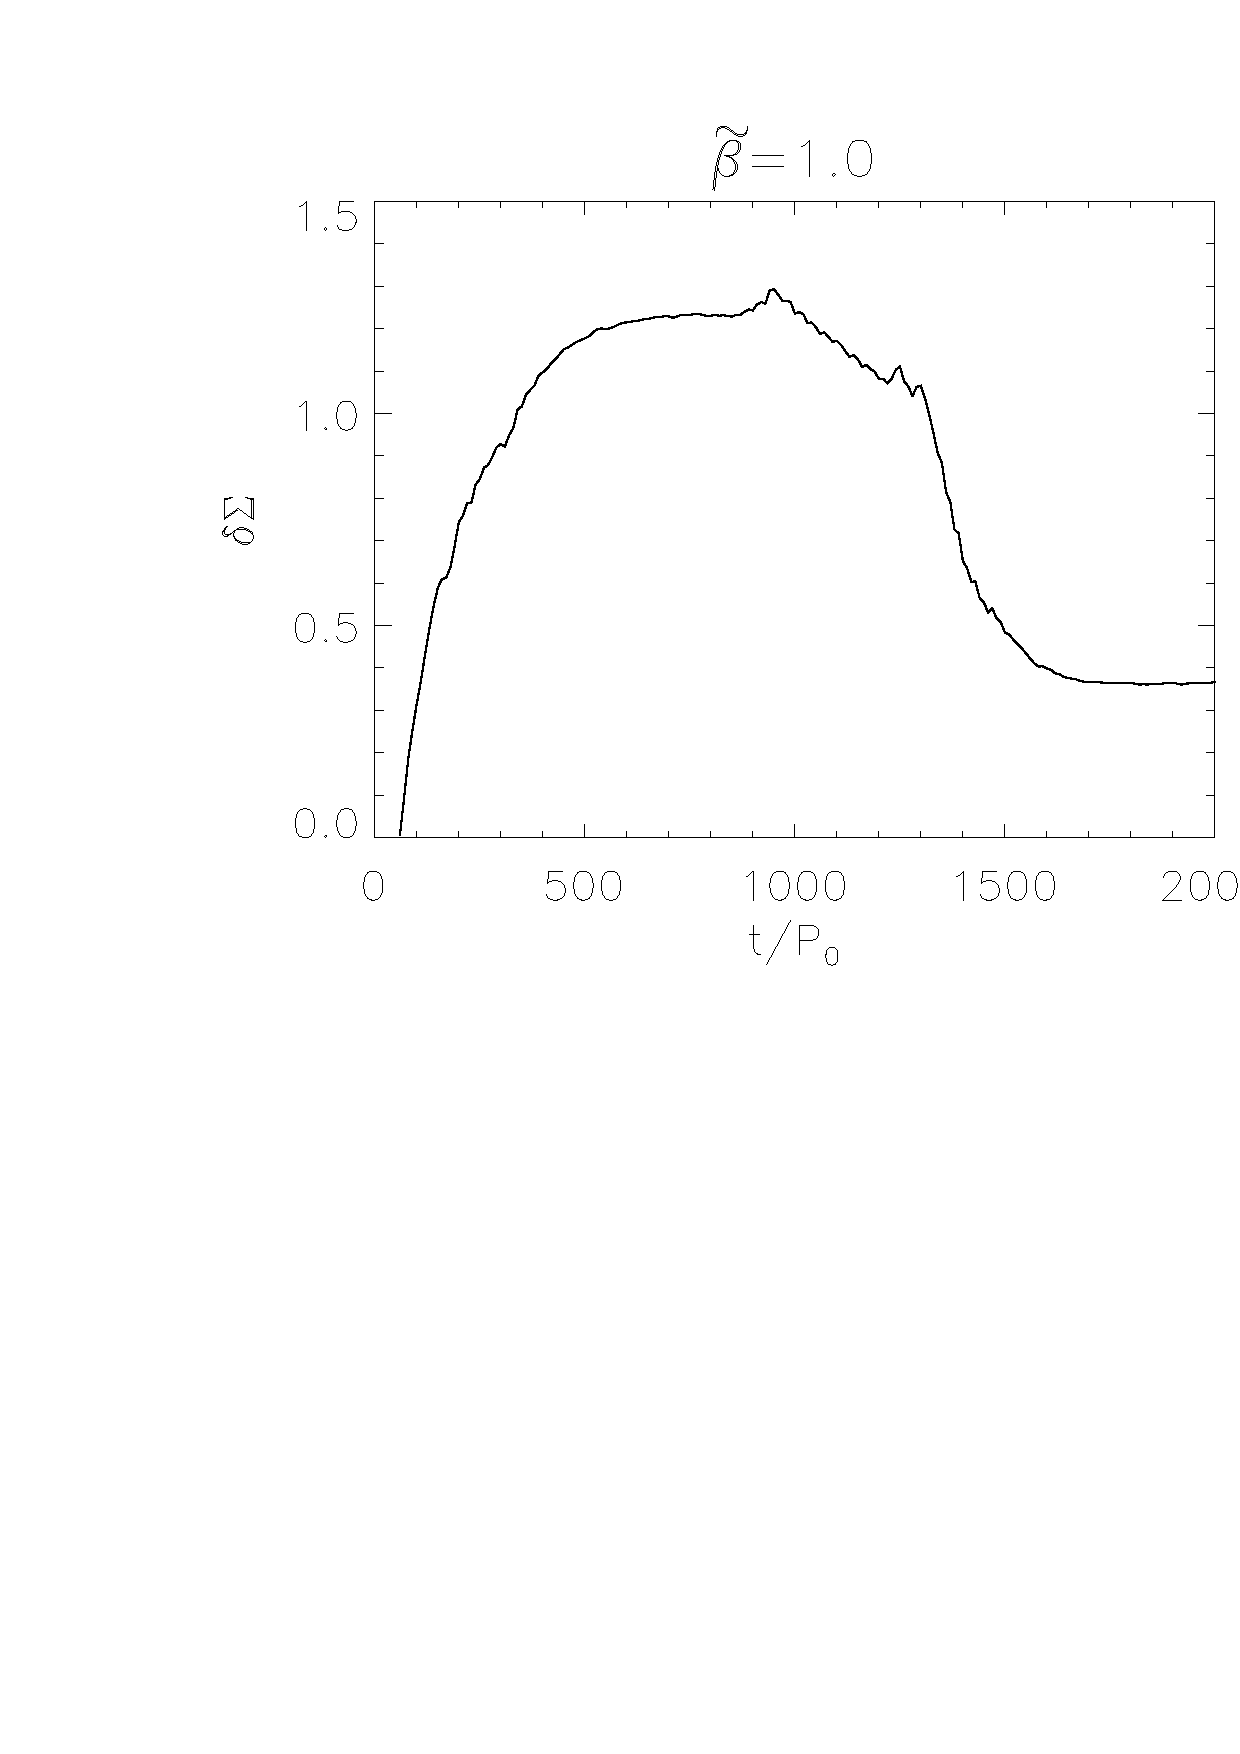
\includegraphics[width=\linewidth]{figures/gap_smoothness}
  \caption{Non-dimensional measure of the surface density gradient at
    the outer gap edge $\tilde\beta=1.0$. During the vortex quasi-steady state
    the gap edge is found to have a large gradient and sharp peak while vortex
    dissipation,
    which occurs at $t\approx1000P_0$ as seen in Fig. \ref{lifetimeplot},
    works to smoothen out the gap edge.
% A large $\delta\Sigma$
 %   corresponds to a more sharply peaked outer gap edge.
    \label{smoothnessplot}}  
\end{figure}


% {\bf It's a good idea to display the smoothening of the outer gap
%   edge with time. 
%   The gap depth parameter correlates
%   well with vortex decay, but its sharp decrease in magnitude gives
%   the impression that the gap is 
%   `filled', which doesn't reflect Fig. \ref{gap_smoothed}. Visually,
%   the gap depth is the same, but the local surface density maximum at
%   the outer gap edge is smoothed. Perhaps we can come up with another
%   way to characterizing the sharpness of the peak? then we can show
%   how this peak is smoothed during vortex decay
% }

% Here, we are interested in the region
% $r>r_p$ since the vortex is located at the outer gap edge. We 
% define a gap depth parameter by averaging the relative surface density
% perturbation within $r\in[r_p,r_e]$ where $r_{e}$ is defined as the
% outer gap radius such that $\langle\Delta
% \Sigma(r_e)/\Sigma(t=0)\rangle_{\phi}=0$.  A more negative gap depth
% parameter correlates with a steeper gap edge. 

% Fig. \ref{gapdepth} shows the evolution of the gap depth parameter
% for $\tilde\beta=1.0$. The magnitude of the gap depth is seen to 
% slowly increase as vortex reaches its maximum amplutude at
% $t\sim1000P_0$, followed by a sharp decrease coincident with vortex 
% decay.  

% \begin{figure}
%   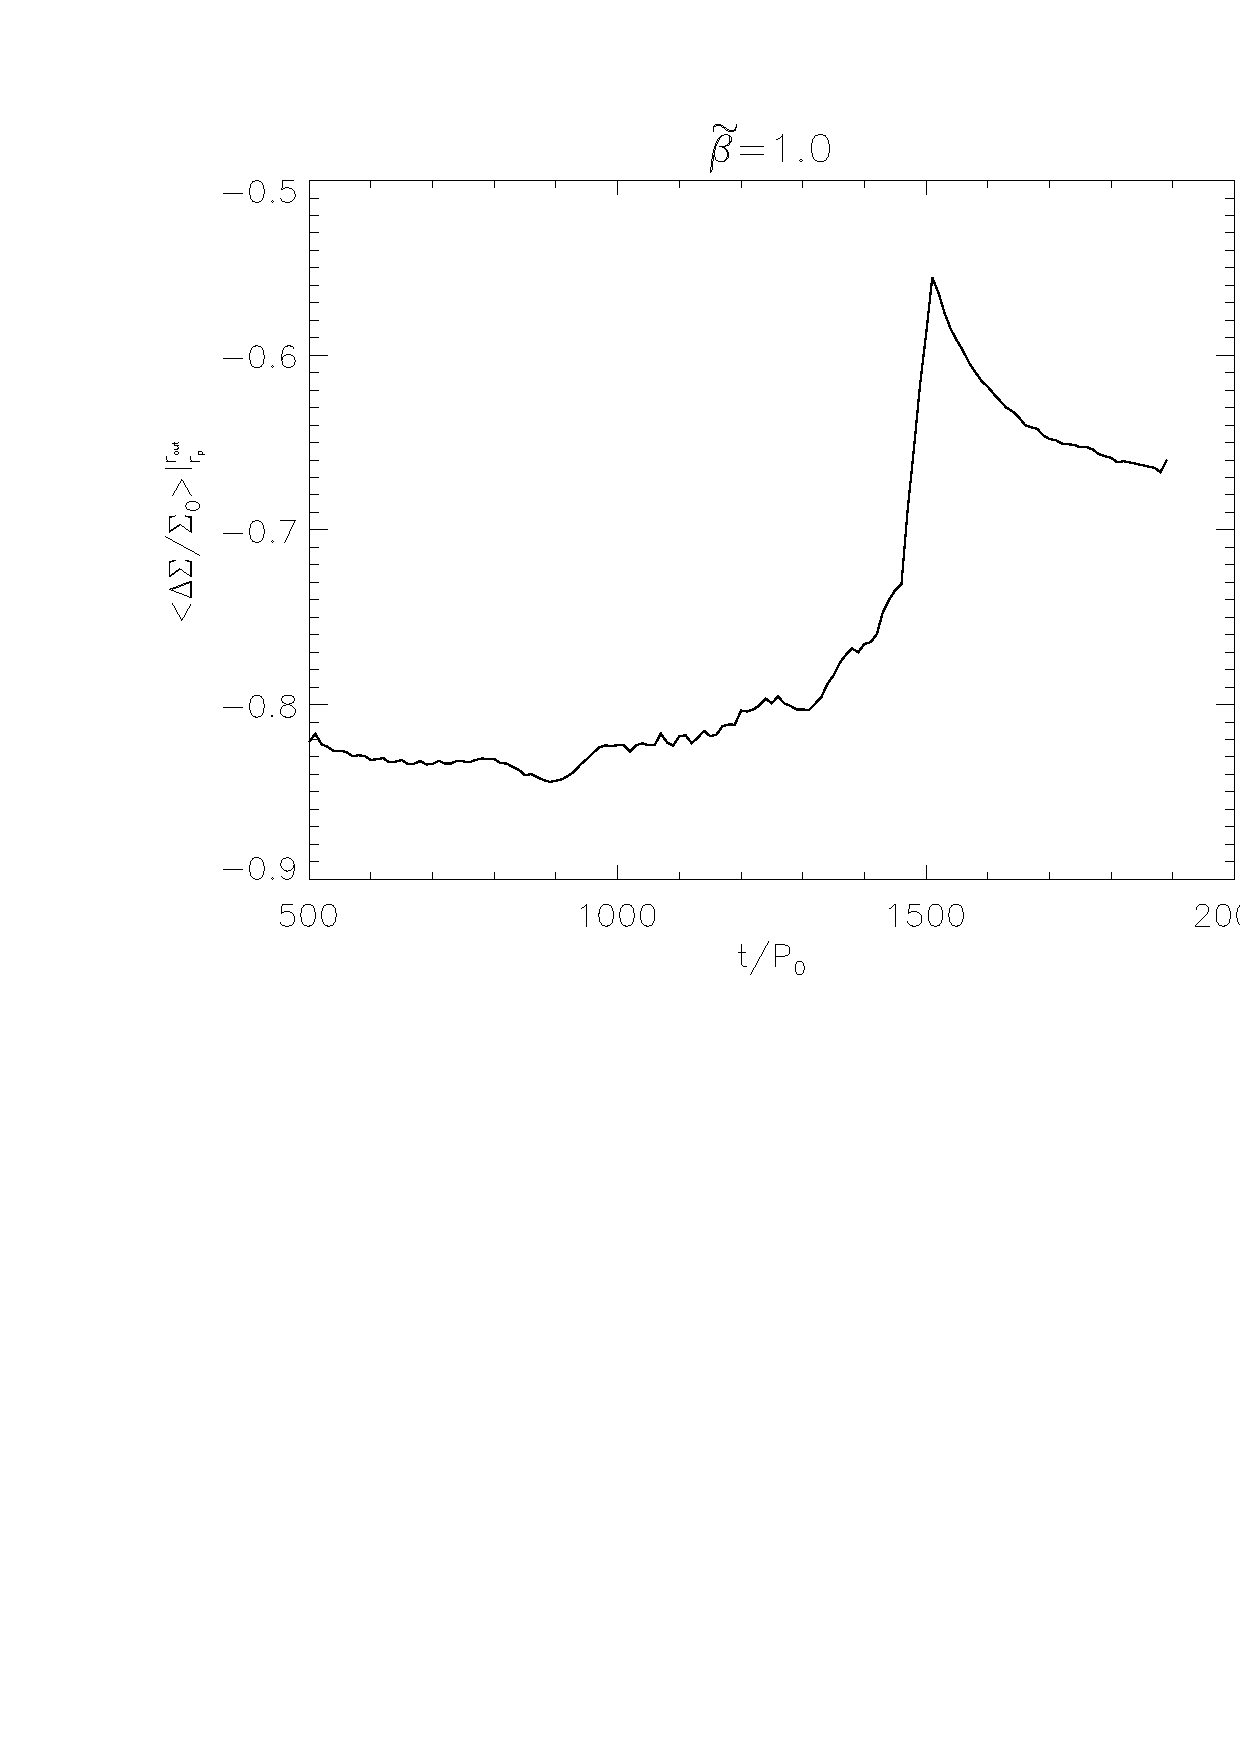
\includegraphics[width=\linewidth]{figures/gapdepth}
%   \caption{Running-time average of the gap depth parameter, defined as
%     the relative surface density perturbation averaged over the
%     outer half of the gap.} \label{gapdepth}
% \end{figure}

\subsection{Vortex lifetimes as a function of cooling
  rate}\label{lifetime_discuss} 
% {\bf the discussion here may need to be changed, depending on
%   updated/new definitions of vortex lifetime. here, i'm assuming we
%   still get the non-monotonic dependence, which may or may not remain
%   true. 
% }

We now examine vortex lifetimes as function of the imposed cooling
times. We define the vortex lifetime, $t_{\mathrm{life}}$, as the time
at which the over-density of the vortex
% to reach $10\%$ of its max overdensity value
returns to $\Delta \Sigma/\Sigma_0\sim1$ \emph{after} reaching maximum
%{\bf correct interpretation?}
 (which is on the order of the
initial over-density associated with the gap formation). 

We plot $t_{\mathrm{life}}$ with respect to cooling times in
Fig. \ref{betaplot}. We also plot $t_{\mathrm{diss}}$: the time elapsed before the
vortex to begins to dissipate (when the $m=1$ surface density
amplitude begins to decay); and $t_{\mathrm{Mach}}$: the time taken
for the average Mach number around the vortex to maximise. 

For fast cooling rates ($\tilde{\beta}\lesssim 1$), the
vortex lifetime is maximised for $\tilde{\beta}\to0$: we find 
$t_{\mathrm{life}} \approx 1300P_0$ for $\tilde{\beta}=0.1$ and 
decreases to $t_{\mathrm{life}} \approx 1100P_0$ for
$\tilde{\beta}=0.5$. This is due to the longer decay timescale with
decreasing $\tilde{\beta}$. For longer cooling times ($\tilde{\beta}\gtrsim
1$) the vortex lifetimes maximises at $\tilde\beta=5.0$ with 
$t_{\mathrm{life}}\approx 1525P_0$.  The other timescales $t_\mathrm{diss}$ and
$t_\mathrm{Mach}$ are less complicated, but still display a
non-monotonic dependence on $\tilde{\beta}$, with a single maximum at
$\tilde{\beta}=1$. 
% his is in comparison with the timescale of intial vortex dissipation which has 
% non-monotonic dependence and a single maxima at $\tilde\beta=5.0$.
%non-monotonic dependence for all timescales

\begin{figure}
  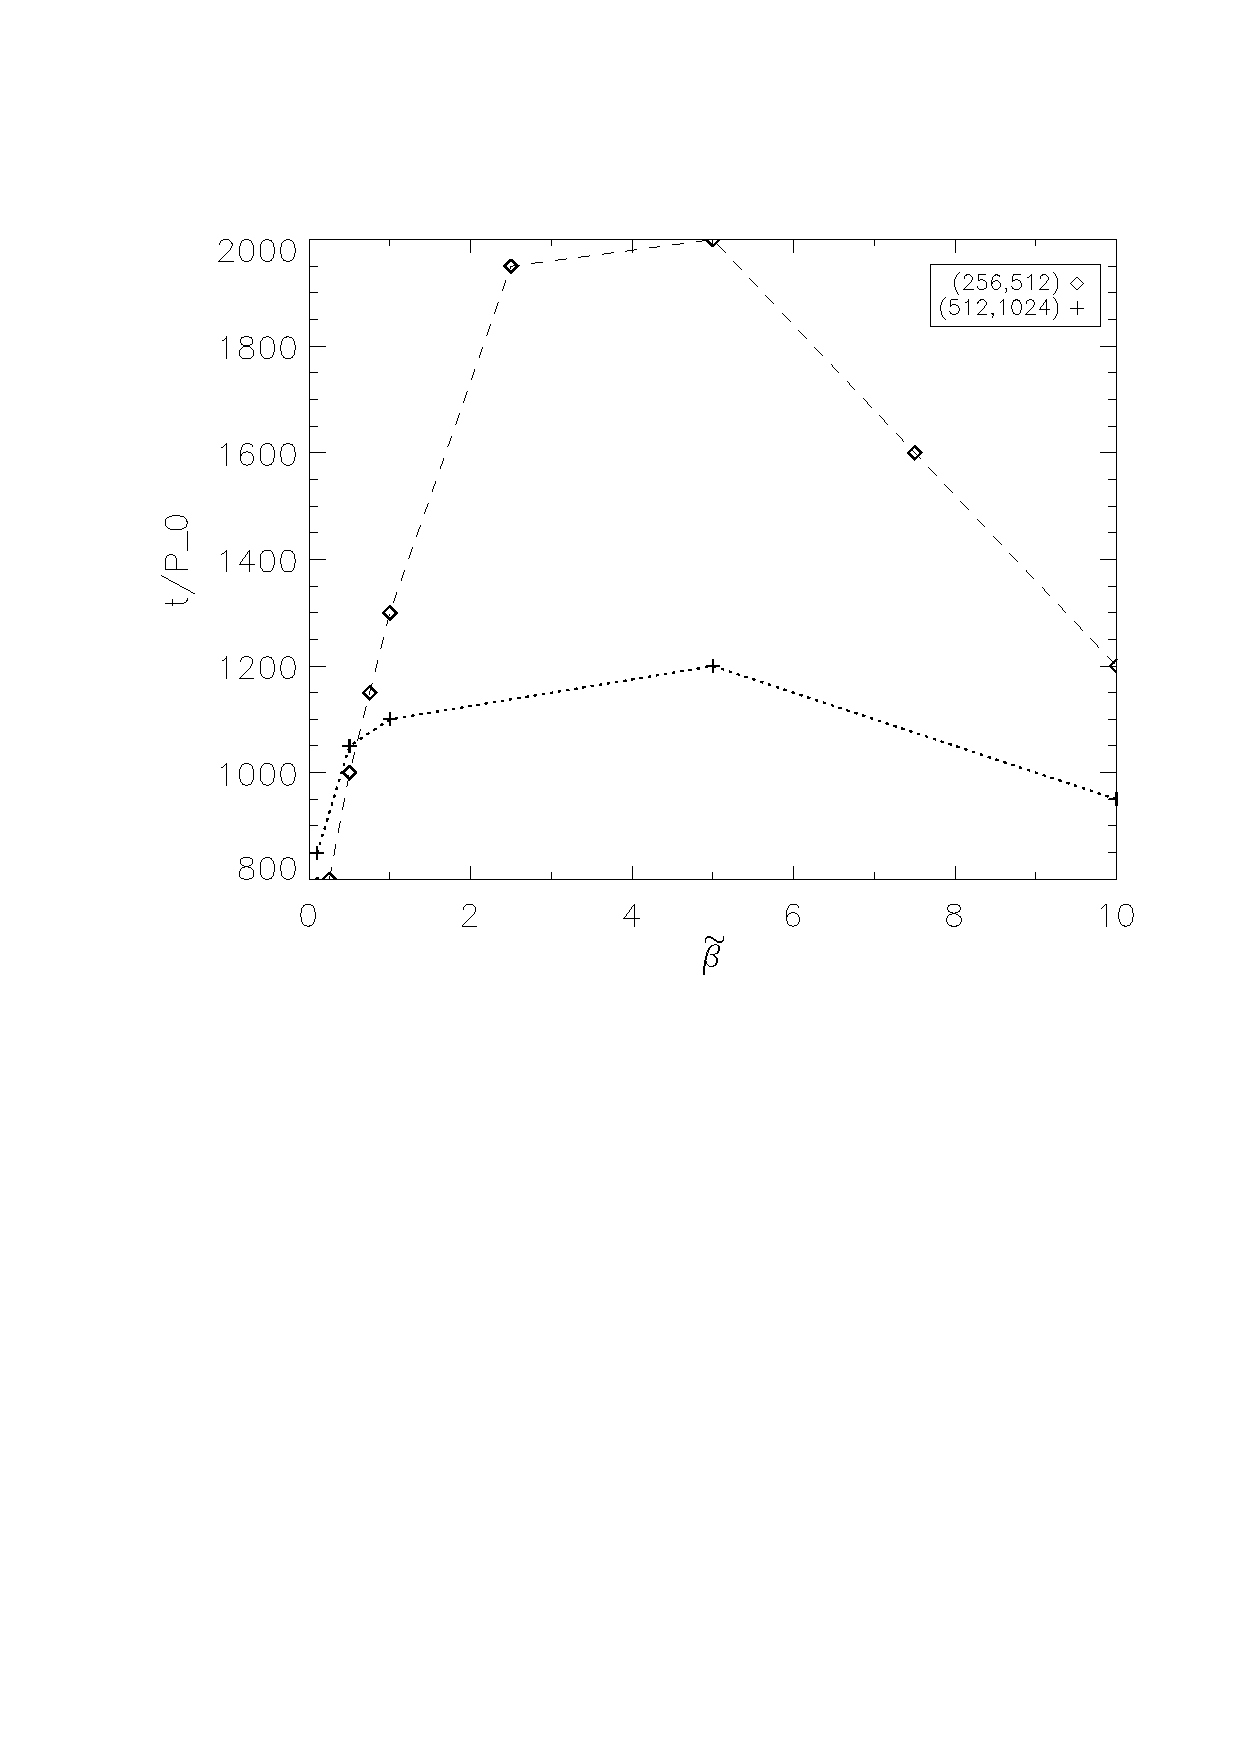
\includegraphics[width=\linewidth]{figures/betaplot}
  \caption{Characteristic timescales associated with vortex evolution, as a function of the cooling
    parameter $\tilde\beta$: time in which the $m=1$
    surface density amplitude begins to decay, $t_\mathrm{diss}$ (black);
    time at which the over-density at the
    vortex centre decreases to $\Delta\Sigma/\Sigma \sim 1$ after
    reaching maximum, $t_\mathrm{life}$ (red);
    and $t_\mathrm{Mach}$ is the time taken
    for the average Mach number around the vortex to maximise
    (blue). \label{betaplot}}  
% {\bf maybe useful to over-plot other timescales,
%      e.g. time taken to reach max mach, time for rossby number to
%      reach zero.}
\end{figure}

In the previous section, we observed that vortices began to decay when
it starts to induce shocks. We therefore suggest the vortex lifetime
is determined the time needed for the vortex to grow to 
sufficient amplitude to induce shocks in the surrounding fluid, and 
the decay timescale itself. The latter was found to shorten 
with increasing $\tilde{\beta}$. However, the former timescale
($t_\mathrm{diss}$), which may be considered as the 
duration of the quasi-steady state, reaches a single maximum with
respect to cooling time. The sum of these two timescales results in the
double-peaked behaviour of $t_\mathrm{life}$ in Fig. \ref{betaplot}. 
% \footnote{The 
%  decay timescale itself is also a factor, but we found this timescale
%  to be much shorter than the duration of the quasi-steady state
%  (Fig. \ref{lifetimeplot}), except at very short cooling times.}. 
We suggest below competing factors that may result in this
non-monotonic dependence of $t_\mathrm{diss}$ on the cooling rate.  

\subsubsection{Factors that lengthen vortex lifetimes}
It has been shown that the amplitude at which the RWI saturates 
increases with the growth rate of the linear instability  
\citep{meheut2013}. Our `planet-off' simulations yield slower growth
rates with increasing cooling times, which suggest weaker vortices are
formed initially with increasing $\tilde{\beta}$. This is consistent
with the present simulations: at the beginning of the 
quasi-steady  state ($t\sim100P_0$) we find the over-density at the
vortex centre is $\Delta\Sigma/\Sigma_0=2.5$ for $\tilde\beta=0.1$ and
$\Delta\Sigma/\Sigma_0=1.48$ for $\tilde\beta=10$.%, both with
%$Ro\simeq-0.15$.   
% {\bf rossby numbers?} 

The growth of the post-merger single vortex is mediated by disc-planet
interaction. However, gap-opening becomes more difficult in a hotter 
disc, and we find the generalised vortensity 
profiles are smoother with increasing $\tilde{\beta}$. This opposes
the RWI. 
%this effect probably becomes less important for very long
% cooling times -> our gap profiles for beta=1, 10 and 100 appear similar
Furthermore, the vortex should reach larger amplitudes to induce
shocks on account of the increased sound-speed.  

These considerations suggest, with increased cooling times, 
it takes longer for the post-merger vortex grow to sufficient
amplitude to induce shocks and dissipate. This factor contributes to a
longer quasi-steady state with increasing $\tilde{\beta}$.       

%{\bf hotter disc $\to$ gap edges less sharp, still true during quasi
%  steady state?: gap edges almost identical in quais-steady but generalized vortensity smoothed out}

\subsubsection{Factors that shorten vortex lifetimes} 
% However, Fig. \ref{lifetimeplot} shows that very long cooling
% times (e.g. $\tilde{\beta}=10$) actually results in a \emph{shorter} vortex
% lifetime. 
Notice in Fig. \ref{lifetimeplot} and Fig. \ref{overdensity}, the vortex 
growth during the quasi-steady state is actually faster for $\tilde{\beta}=10$
than for $\tilde{\beta}=5$. 
For example, at $t\sim 500P_0$ the vortex with    
$\tilde{\beta}=10$ has a larger 
amplitude than for $\tilde{\beta}=5$. This is also reflected in Fig. \ref{machplot}, where the
Mach number reaches its maximum value sooner for $\tilde{\beta}=10$
than for $\tilde{\beta}=5$.  

This observation is consistent with the RWI being favoured by 
higher temperatures \citep{li00,lin12c} through the perturbations 
(as opposed to its effect through the set up of the gap profile
discussed previously),
which corresponds to longer cooling times in our case. 
While our `planet-off' simulations indicate this is unimportant for
the linear instability, it may have contributed  
significantly to the vortex growth during quasi-steady state at very
long cooling times (e.g. $\tilde{\beta}=10$). This effect shortens the
vortex lifetime by allowing it to grow faster and induce shocks
sooner.  

%This effect can be seen in Mach number around the vortices where the
%growth of Mach number with respect to time is increasing with cooling rate.
%Thus the intially weaker formed vortices for higher cooling rate grow
%substantialy faster than the sound speed and can shock the system in earlier
%times.
%While our `planet-off' simulations show 
%This may be attributed to the higher temperature
%reached in the latter case 
%
%($h\simeq 0.07$) in comparison with the former
%($h\simeq 0.06$), since \cite{li00} showed that the RWI is favoured by
%larger disc temperature.  
